\documentclass[aps,pre,twocolumn,showpacs,showkeys,superscriptaddress,floatfix]{revtex4-1}
 %\pdfoutput=1 \input epsf

\usepackage[utf8]{inputenc}
\usepackage[english]{babel}
\usepackage{hyperref}

\usepackage{amsmath}
\usepackage{amssymb}
\usepackage{amscd}
\usepackage{mathtools}

\usepackage{color}
\usepackage{graphicx}
\usepackage{subfigure}

\usepackage{upgreek}
\usepackage{dcolumn}
\usepackage{natbib}

\DeclareMathOperator{\erfc}{erfc}

\newcommand{\rmd}{{\mathrm d}}
\newcommand{\rme}{{\mathrm e}}
\newcommand{\dbar}{{\mathchar '26 \mkern-11mu {\mathrm d}}}

\renewcommand{\vec}[1]{{\boldsymbol {#1}}}
 %  \usepackage{showkeys}

\begin{document} 

\title{The interaction between Actin and Myosin-II, the flashing ratchet}
\author{Pieter Baerts}
%\author{Christian Maes}
\affiliation{KU Leuven, Instituut voor Theoretishe Fysica, Celestijnenlaan 200D, B-3001 Leuven, Belgium}
\author{Jiří Pešek}
\author{Herman Ramon}
\affiliation{KU Leuven, BIOSYST-MeBioS, Kasteelpark Arenberg 30, B-3001 Leuven, Belgium}

\begin{abstract}
We present a model for the movement of a myosin-II molecular motor along a straight actin filament, in which the heads of the motor are subjected to a flashing ratchet potential. This simple model already features the force-velocity relation and aspects of mechanosensing. We also investigate the energy input from the chemical ATP cycle and its dependence on external loads on the motor.  
\end{abstract}

\maketitle 

\section{Introduction}

The cytoskeleton of a cell serves two main purposes, being transporting large vesicles and governing the cell's motility, i.e. the ability of the cell to move and change its shape. 
It mainly consists of long semi-flexible polymers and molecular motors. 
These motors contain several heads that are able to bind to polymer filaments and walk along them. 
The mechanism for walking relies both on a chemical cycle in the motor's head and on the asymmetry of a periodic and electrostatic potential along the length of such a polymer. The part of the cytoskeleton that is mainly responsible for the motility of the cell is the actin-myosin cortex and it will serve as the exemplary system in this paper.

The aims of this study are to reproduce certain features of molecular motors in our simple ratchet model, with constant chemical rates, and to relate the force-velocity relation to the mean force generated by the ratchet and to tension in the motor.
We introduce an efficiency of the motor that is not related to transport, but solely to the net supply of energy provided by the chemical cycle 
and investigate how this chemical efficiency changes when the motor experiences an external load.

The chemical cycle is driven by ATP molecules that can attach to a motor head, causing it to change the charge of the head and consequently loosen its bond with the polymer filament. 
When bound to a motor head, the ATP molecule will hydrolyze to ADP and release a phosphate. 
It this state, the head can attach to the polymer again, ADP will be released from the motor head and the chemical cycle can start over. 
Hence, the chemical state of a motor head will determine how strongly it can be coupled to a cytoskeletal filament. 


Cytoskeletal polymers exhibit a sequence of monomers that cause a periodical structure. 
Furthermore, these monomers are polarized, so that when chained together in a polymer, they give rise to a symmetric, ratchet-like, electrostatic potential along the length of the filament. 
An example of such a potential is shown in figure \ref{fig:energy}. 
The heads of a motor, too, carry an electric charge and therefore they will feel the ratchet potential of the filaments. 
In the attached state, the motor will tend to be close to minimal potential energy. 
However, when the chemical state of the head changes, so does its molecular structure and charge. 
As mentioned earlier, this causes the bond between the head and a filament to either strengthen or loosen. 
Therefore the head will experience a ratchet potential that is flashing in time, changing the amplitude of the potential from high to low.


When tightly bound, the head will most probably be very close to a minimum in the ratchet potential, while in the unbound state, it is easier for the motor to diffuse over a larger distance. 
However, because of the asymmetry of the ratchet, the motor will be biased to explore one side of the ratchet rather than the other. 
Therefore, the motor will more likely jump to an adjacent period of the ratchet potential in the preferred direction, indicated by the asymmetry of the potential. 
This will eventually lead to ballistic motion of the motor on long timescales.

This mechanism motivates the assumptions of ratchet models, being the fact the the motor heads interact with a periodic asymmetric potential that changes depending on the chemical state of the head. 
Such ratchet models have been studied extensively in the context of molecular motors \cite{reimann2002brownian,astumian1994fluctuation,astumian1996mechanochemical,julicher1997modeling,Reimann2002introduction,julicher1997spontaneous,peskin1995correlation,huxley1969mechanism,huxley1971proposed}.
The models that have been used in these studies are very similar to each other but often differ in some basic assumptions.
The specific model that we have studied is presented in section \ref{sec:ratchet}. 
It has the important trait that the chemical rates do not depend on spacial degrees of freedom and motor heads can attach and detach anywhere along the polymer filament.
Furthermore, the rates do not dependent on external forces on the motor but solely on concentrations of chemicals involved in ATP hydrolysis. We assume that constant concentrations are maintained in the environment. 
The type of motor that we will be studying is non-muscle myosin II, which have a small number of heads \cite{pollard1982structure}. 
These motors are believed to be crucial the motility in most eukaryotic cells \cite{vicente2009non}.
For larger myosin motors, like the ones in muscle cells, mean-field calculations have lead to analytic results for the force-velocity relation \cite{julicher1997modeling}.
In experimental studies with synthetic myosin motors, the number of heads per motor is also much higher than in non-muscle cells. 
Therefore, the results for large motor play a very important role in interpreting and understanding those in-vitro experiments \cite{brown2009cross-correlated}.
For motors with fewer heads, mean-field methods are not suitable and numerical simulations prove to be useful.
In sections \ref{sec:velocity} and \ref{sec:force-velocity} we will describe the movement of this motor-polymer system in detail by means of computational simulations.


Another important aspect of molecular motors is their ability to convert chemical energy into mechanical work \cite{astumian1996mechanochemical}.
The chemical cycle of ATP hydrolysis consists out of many consecutive reactions and after one full cycle a net amount of energy is provided to the motor head.
However, often this cycle is represented by only two states, e.g. ATP bound and ADP bound, 
in which case a stochastic process on these states always satisfies detailed balance and no chemical energy can be extracted. 
In other words, the gain of one reaction is canceled by the cost of the following reaction.
On the other hand we do not want any redundant degrees of freedom in our description since we are not really interested in the full chemical details of the process.
In section \ref{sec:energie}, we will look at an alternative way of interpreting the chemical input by measuring the differences in potential energy in each jump and we define a chemical efficiency.
In section \ref{sec:perturb} we provide a perturbative calculation to validate and understand some features of this chemical efficiency and how it changes when the motor is under external load.


Lastly, in section \ref{sec:mechanosensing}, we look at the coupling of the motor to an elastic environment.
Earlier studies have shown that motors are able to sense the stiffness of their environment and that they can adapt the active forces that they generate \cite{stam2015isoforms,albert2014stochastic}.
In those studies the rates did depend on the load on the motor. We show computationally that a motor in our simple ratchet model with constant rates behaves similarly.


\section{The Ratchet model}
\label{sec:ratchet}
In order to investigate the movement of myosin along the actin filament and the forces it generates, we consider the following one dimensional model.
Firstly, we assume that the rigidity of the actin polymer and myosin backbone is high enough that their elongations can be neglected.
Secondly, we assume that all myosin heads are attached directly to the myosin backbone at fixed equidistant positions, see figure~\ref{fig:ratchet setup}.
These simplifications allow us to model both the motor and the filament as point particles undergoing overdamped diffusion in the inter-cellular environment \cite{vanKampen1981stochastic}.
Moreover, each myosin head has an internal state, which represent its chemical state, 
i.e. whether there is an ATP bounded or not to the myosin head. 
\begin{figure}[t]
\centering
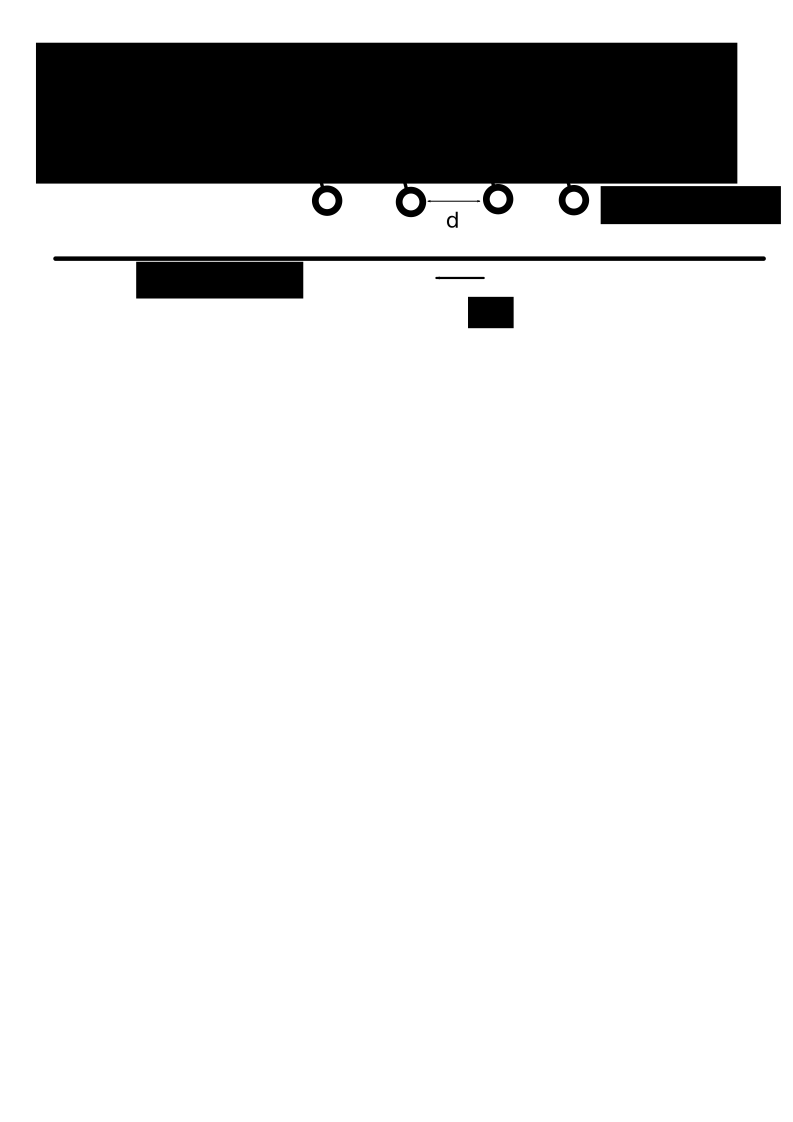
\includegraphics[width=0.45\textwidth,height=!]{ratchet_illustration}
\caption{
\label{fig:ratchet setup}
In this illustration the basic setup is depicted.  
The backbone of the myosin motor is shown with four heads that are equidistantly spaced with $d$ denoting their respective distance. 
The load $F_\text{load}$ is applied only on myosin and the actin filament is freely diffusing. 
} 
\end{figure}

The dynamics of positions is described by coupled overdamped Langevin equations 
\begin{align}
&\begin{multlined}[b]
\rmd x_\text{M} = 
\frac{1}{\gamma_\text{M}} \left[ - \nabla_\text{M} V_t(x_\text{M}(t) - x_\text{A}(t)) + F_\text{load} \right] \; \rmd t 
\\ 
+ \sqrt{ \frac{2 k_B T}{\gamma_\text{M}} } \; \rmd W_\text{M} ,
\end{multlined}
\label{eq:eom_M} \\
&\begin{multlined}[b][.42\textwidth]
\rmd x_\text{A} = 
- \frac{1}{\gamma_\text{A}} \nabla_\text{A} V_t(x_\text{M}(t) - x_\text{A}(t)) \; \rmd t 
\\
+ \sqrt{ \frac{2 k_B T}{\gamma_\text{A}} } \; \rmd W_\text{A} ,
\end{multlined}
\label{eq:eom_A}
\end{align}
where $x_\text{M}$ ($x_\text{A}$) denote the position of myosin (actin polymer), 
$\gamma$ is the Stokes drag,
$T$ is the absolute temperature of the environment,
$W$ denotes the Wiener process,
$F_\text{load}$ is an external load on the motor, 
and the interaction potential $V_t$ represents the overall ratchet interaction, which is a sum over individual contributions from all motor heads,
\begin{equation}
V_t(x) = \sum\limits_{i=0}^{N-1} \zeta_t(i) \, V_\text{r} (x - i \, d ), 
\label{eq:ratchet_interaction}
\end{equation}
where $d$ is the distance between myosin heads, 
$N$ is the number of heads per motor,
$\zeta_t(i)$ represents the internal state, see bellow, 
and $V_\text{r}$ is the periodical ratchet potential, see figure~\ref{fig:energy},
\begin{equation}
V_\text{r}(x) =  \begin{cases}
        V_\text{r}(x+\ell) & x < 0 \\[1ex] 
        \displaystyle \frac{ V x }{ a \ell } & 0 \leq x < a \ell \\[2ex]
        \displaystyle \frac{ V (\ell-x) }{ (1-a) \ell } & a \ell \leq x < \ell \\[2ex]
        V_\text{r}(x-\ell) & \ell \leq x  
   \end{cases} ,
   \label{eq:ratchet_potential}
\end{equation}
with total height $V$,
period $\ell$ 
and skewness parameter $a \in [0,1]$. 
\begin{figure}[t]
\centering
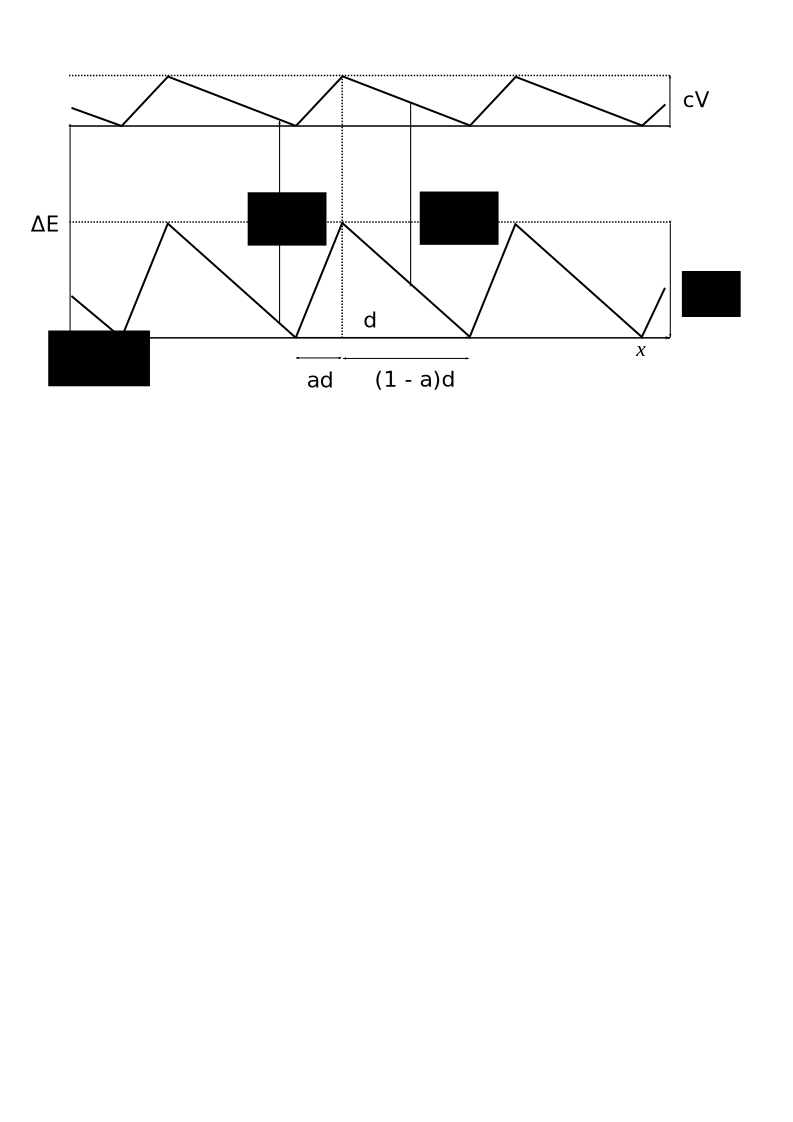
\includegraphics[width=0.45\textwidth,height=!]{energy}
\caption{
\label{fig:energy}
Energy landscape for the myosin's head.
The basic interaction with actin polymer is via Ratchet potential with the potential height $V$, period $\ell$ and skewness parameter $a$.
The transition between ATP \emph{bound} and \emph{unbound} state is govern by rates $k_\text{bind}$, $k_\text{unbind}$ 
and is associated with the chemical energy $\Delta E$.
In the \emph{bound} state the ratchet potential is scaled down by factor $c$. 
}
\end{figure}

The dynamics of internal state of heads is governed by continuous time Markov process. 
Here, the internal state represents whether ATP is \emph{bound} or \emph{unbound} to the myosin head. This specifies the electrostatic properties of the head which will determine the amplitude of the interaction potential with the actin filament.
No effective dependencies on position or external forces are imposed on the dynamics of the chemical cycle. 
Work done by external forces is dissipated through the diffusion processes of the motor and polymer, see section \ref{sec:energie}.
This is a simplification over the full chemical network governing the internal states of myosin \cite{Bierbaum2011,Bierbaum2013},  
which focuses only on the long lasting states that significantly change the myosin's head physical properties.
Namely, we look at states where ADP is bounded and where there is no molecule bound to myosin head as escape rates from those states are small with respect to other transitions \cite{Bierbaum2011},%TODO 
for which the estimated free energy landscapes \cite{Nie2014,nie2014conformational} very well reflect the changes in  conformation and electric charge of the myosin head \cite{barterls1993myosin}.
In order to obtain the transition rates between these to two states, we start from the three state model introduced by Albert et al. \cite{albert2014stochastic},
which we further simplify by unifying the state corresponding to the hydrolized ATP (i.e. ADP+P) and ADP with P released state as this process occurs on much shorter time-scale than other transitions.
Lastly, as the internal state reflects the chemical state of the head rather then the act of binding to actin itself,
we assume that external load have little influence on the associated rates but rather opposes the underlying free energy landscape. 
These considerations are reflected in the assumption the rates $k_\text{bind}$, $k_\text{unbind}$ independent of the load, 
but they depend on the concentrations of the relevant chemical species present in ATP hydrolysis. 
More specifically $k_\text{bind}$ is proportional to $[\text{ATP}]$ while $k_\text{unbind}$ is inversely proportional to $[\text{ADP}]$ and $[\text{P}_\text{i}]$.
The dynamics is then represented by dichotomous continuous times Markov process with constant rates,
\begin{equation}
\zeta_t = 1 \overset{k_\text{bind}}{\underset{k_\text{unbind}}{\rightleftarrows}} \zeta_t = c ,
\label{eq:transition}
\end{equation}
where $c\in\left[0,1\right]$ determines the amplitude of the ratchet potential when the motor is loosely bound to the filament, 
which we use as an approximation for changes in the free energy landscape \cite{Nie2014,nie2014conformational}.
While both the diffusion and the jump process are in equilibrium, the mechanism of the flashing ratchet brings the combined system out of equilibrium, leading to the movement of the motor in a preferred direction, given by the asymmetry of the filament. 

Figure~\ref{fig:ratchet setup} depicts the whole setup of the system
and figure~\ref{fig:energy} depicts the dynamics involved in flashing ratchet. 
Table \ref{tab:parameters} lists the values of the parameters used in this model. 
Some of them were taken from the literature while others were fitted to give a realistic mean velocities and stall force for the myosin II. 
The friction coefficients were calculated with Stokes' law \cite{Broersma1960,Broersma1981}, using the known dimensions of the molecules \cite{yogurtcu2012mechanochemical,pollard1982structure} and the viscosity of the extracellular medium \cite{li2004diffusion}.
\begin{table}[t]
\centering
\begin{ruledtabular}
\begin{tabular}{lcdcc}
Parameter & Symbol & \multicolumn{1}{c}{Value} & Units & Source\\
\hline
Thermal energy& $k_B T$ & 4.28 & pN nm & --- \\
Number of heads& $N$ & 4 & --- & \cite{pollard1982structure}\\
Head's spacing& $l$ & 15 & nm & \cite{pollard1982structure}\\
Step length& $d$ & 8 & nm & \cite{vilfan2003instabilities}\\
Binding rate& $k_\text{unbind}$ & 40 & s$^{-1}$ & \cite{albert2014stochastic} \\
Detaching rate& $k_\text{bind}$ & 80 & s$^{-1}$ & \cite{albert2014stochastic} \\
Skewness& $a$ & 0.25 & --- & ---\\
Potential amplitude& $V$ & 40 & pN nm & ---\\
Potential scaling& $c$ & 0.3 & --- & \cite{Nie2014, nie2014conformational}\\
Chemical energy gap & $\Delta E$ & 30.4 & pN nm & \cite{gajewski1986thermodynamics}\\
Motor friction& $\gamma_{m}$ & 0.66 & pN $\upmu$s nm$^{-1}$ & \cite{Broersma1960,Broersma1981} \\ %TODO
Actin friction& $\gamma_{a}$ & 0.97 & pN $\upmu$s nm$^{-1}$ & \cite{Broersma1960,Broersma1981} \\ %TODO
\end{tabular}
\end{ruledtabular}
\caption{
\label{tab:parameters}
Table of all parameter values and a reference to their source.
}
\end{table}

\subsection{Other setups}
While the previous setup is the most studied \cite{reimann2002brownian,astumian1994fluctuation,finer1994single,julicher1997modeling,kishino1988force,peskin1995correlation,saito1994movement},
it's aim is to characterize the transport induced by molecular motors.
However, recent experiments show that myosin II role is mainly for cross-linking the cytoskeleton and consequently producing an active tension inside the network \cite{ma2012nonmuscle}.
Here we present two natural extensions of the previous setup suitable for investigation of the behavior of the molecular motor inside of the network.

\subsubsection{Tug of war}
\label{sec:load_on_fil}
The first extension is that the motor is interacting with two, rather then one, anti-parallel actin filaments. 
Consequently, the external load is now applied directly at filaments instead directly at the motor.
This setup is shown in figure \ref{fig:tug_F_illustration}. 
\begin{figure}[t]
\centering
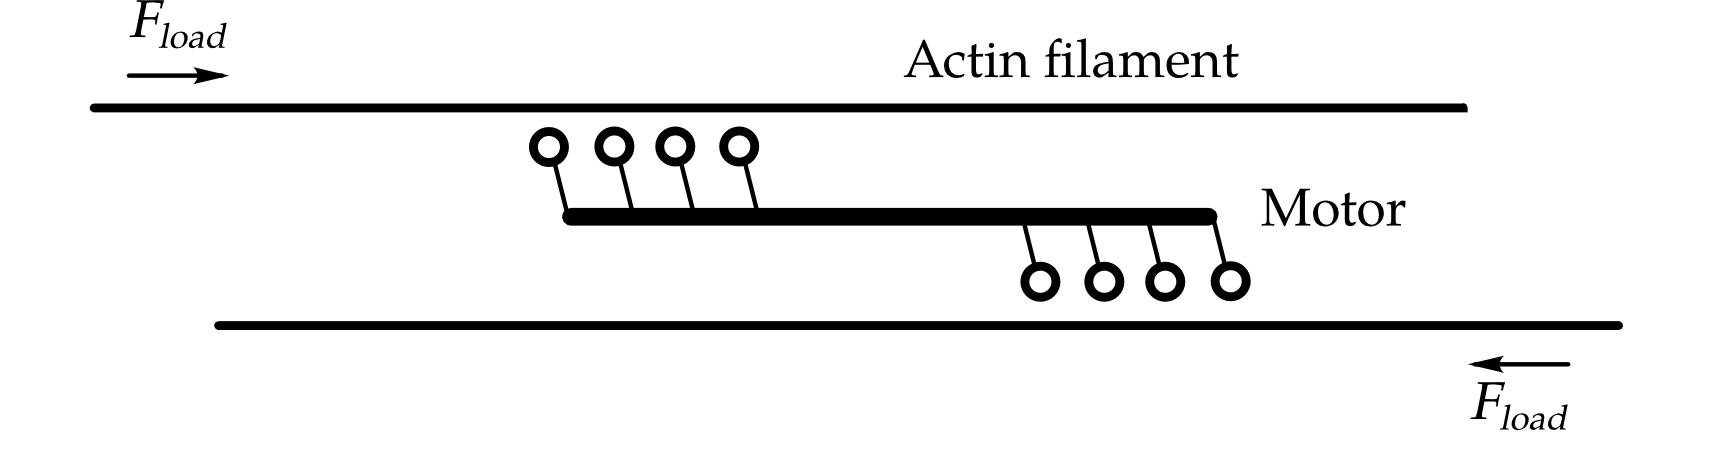
\includegraphics[width=0.45\textwidth,height=!]{tug_F_illustration}
\caption{
\label{fig:tug_F_illustration}
Setup of a motor interacting with two actin filaments that experience equal but opposite loads.
}
\end{figure}

This means that we have now two filaments, denoted by subscript ${\text{A}_1}$ and ${\text{A}_2}$ respectively,
subjected to free diffusion and external load $F_\text{load}$
which are interacting with the myosin II motor via the ratchet potential~\eqref{eq:ratchet_interaction}. 
This lead to equations of motion 
\begin{equation}
\begin{gathered}
\begin{multlined}[b][.45\textwidth]
\rmd x_\text{M} = 
- \frac{1}{\gamma_\text{M}} \bigl[ \nabla_\text{M} V_t(x_\text{M}(t) - x_{\text{A}_1}(t)) 
\\
+ \nabla_\text{M} V_t(x_{\text{A}_2}(t) - x_\text{M}(t)) \bigr] \; \rmd t 
+ \sqrt{ \frac{2 k_B T}{\gamma_\text{M}} } \; \rmd W_\text{M} ,
\end{multlined}\\
\begin{multlined}[b][.45\textwidth]
\rmd x_{\text{A}_1} = 
\frac{1}{\gamma_\text{A}} \left[ - \nabla_{\text{A}_1} V_t(x_\text{M}(t) - x_{\text{A}_1}(t)) + F_\text{load} \right] \; \rmd t 
\\
+ \sqrt{ \frac{2 k_B T}{\gamma_\text{A}} } \; \rmd W_{\text{A}_1} ,
\end{multlined}\\
\begin{multlined}[b][.45\textwidth]
\rmd x_{\text{A}_2} = 
\frac{1}{\gamma_\text{A}} \left[ - \nabla_{\text{A}_1} V_t(x_{\text{A}_2}(t) - x_\text{M}(t)) - F_\text{load} \right] \; \rmd t 
\\
+ \sqrt{ \frac{2 k_B T}{\gamma_\text{A}} } \; \rmd W_{\text{A}_2} ,
\end{multlined}
\end{gathered}
\label{eq:eom_two_actins}
\end{equation}
where the anti-alignment of polymers in substitution of $-x$ instead of $x$ for the second polymer in the argument of the ratchet potential~\eqref{eq:ratchet_interaction}.

Note that due to the symmetry of the setup the mean velocity of the myosin is inherently zero,
\begin{multline*}
\left\langle v_\text{M} \right\rangle 
= - \frac{1}{\gamma_\text{M}} \bigl[ 
\left\langle \nabla_\text{M} V_t(x_\text{M}(t) - x_{\text{A}_1}(t)) \right\rangle
\\ 
+ \left\langle \nabla_\text{M} V_t(x_{\text{A}_2}(t) - x_\text{M}(t)) \right\rangle 
\bigr] 
\\
= - \frac{\gamma_\text{A}}{\gamma_\text{M}} \left[ 
\left\langle v_{\text{A}_1} \right\rangle 
+ \left\langle v_{\text{A}_2} \right\rangle 
\right]
\equiv 0 . 
\end{multline*}

\subsubsection{Elastic environment}
\label{sec:environment}
As polymers inside the cytoskeleton are usually thoroughly interconnected rather then freely diffusing \cite{blanchoin2014actin,ennomani2016architecture},
we can opt for an alternative approach.
Rather then applying an external load we attach filaments to fixed points by a spring with a constant $k$, similar to \cite{albert2014stochastic}. 
These points represent points of interaction with the rest of the network while the spring constant $k$ represents the elastic properties of the full network. 
The myosin motor is again interacting with two filaments that are arranged in an anti-parallel fashion. 
Hence, similar to the previous case, it will no longer have a preferred direction to move in and consequently its mean velocity will be zero. 
The observable of interest is now the mean force that the motor applies to the filaments, 
which is measured through the extension of the springs attached to the filaments,
and which represent the active tension in the network produced by the single myosin molecule. 
This setup is sketched in figure \ref{fig:tug}. 
\begin{figure}[t]
\centering
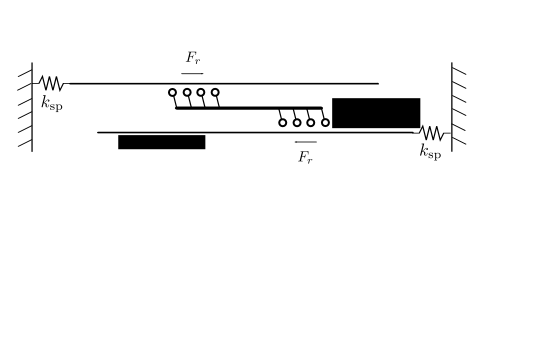
\includegraphics[width=0.45\textwidth,height=!]{tug}
\caption{
\label{fig:tug}
Illustration of a motor pulling on two actin filament that are each connect to a wall by a spring.
}
\end{figure}

The equations of motion are then just a modification of \eqref{eq:eom_two_actins}  
\begin{equation}
\begin{gathered}
\begin{multlined}[b][.45\textwidth]
\rmd x_\text{M} = 
- \frac{1}{\gamma_\text{M}} \bigl[ \nabla_\text{M} V_t(x_\text{M}(t) - x_{\text{A}_1}(t)) 
\\
+ \nabla_\text{M} V_t(x_{\text{A}_2}(t) - x_\text{M}(t)) \bigr] \; \rmd t 
+ \sqrt{ \frac{2 k_B T}{\gamma_\text{M}} } \; \rmd W_\text{M} ,
\end{multlined}\\
\begin{multlined}[b][.45\textwidth]
\rmd x_{\text{A}_1} = 
\frac{1}{\gamma_\text{A}} \bigl[ - \nabla_{\text{A}_1} V_t(x_\text{M}(t) - x_{\text{A}_1}(t)) 
\\
- k \left( x_{\text{A}_1}(t) - x_{\text{A}_1}(0) \right) \bigr] \; \rmd t 
+ \sqrt{ \frac{2 k_B T}{\gamma_\text{A}} } \; \rmd W_{\text{A}_1} ,
\end{multlined}\\
\begin{multlined}[b][.45\textwidth]
\rmd x_{\text{A}_2} = 
\frac{1}{\gamma_\text{A}} \bigl[ - \nabla_{\text{A}_1} V_t(x_{\text{A}_2}(t) - x_\text{M}(t))
\\
- k \left( x_{\text{A}_2}(t) - x_{\text{A}_2}(0) \right) \bigr] \; \rmd t 
+ \sqrt{ \frac{2 k_B T}{\gamma_\text{A}} } \; \rmd W_{\text{A}_2} ,
\end{multlined}
\end{gathered}
\label{eq:eom_two_actins_no_load}
\end{equation}
where the load is replaced by the force caused by springs and the reference point for the springs is chosen as their position at the initial time. 

\subsection{Numerical method}

We use an Euler-Maruyama integration scheme to stochastically evolve the systems from a randomised initial configuration \cite{kloeden1989survey,maruyama1955continuous}. 
Results are obtained after both ergodic and ensemble averaging, up to a minimal time of $1s$ and over $100$ or more independent copies.    

\section{Mean velocity}
\label{sec:velocity}
At first, we study the mean velocity $\langle v\rangle$ of the motor with four heads with respect to the filament for different values of scaling factor $c$, see figure~\ref{fig:c_v}.
We see that mean velocity has maximum at $c=0$ and goes to zero when $c$ approaches $1$. 
This is to be expected since $c=1$ corresponds the equilibrium, where there is no difference between the two internal states, cf.~\eqref{eq:transition},
on the other hand $c=0$ corresponds to the biggest discrepancy between those two states. 
\begin{figure}[t]
\centering
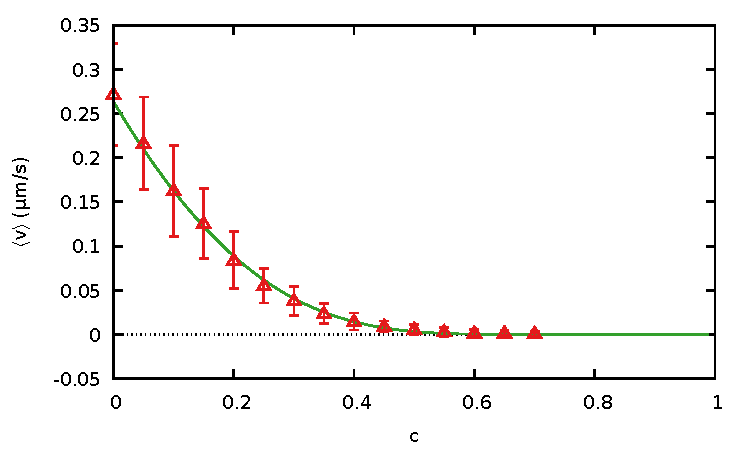
\includegraphics[width=0.45\textwidth,height=!]{c_v_4heads}
\caption{
\label{fig:c_v}
Mean velocity $\langle v \rangle$ of the motor relative to the actin filament for $c \in (0,1)$.
The mean velocity rapidly decreases towards the $0$ as we approach equilibrium, $c \to 1$.  
Green line correspond to the fit $ \left\langle v \right\rangle \propto \exp ( - \frac{\alpha}{1-c} ) $.
%The dependency is guessed, unfortunately I don't have any argument to support it. 
} 
\end{figure}


Secondly, the mean velocity also depends on the concentration of ATP through the unbind rate. 
In this setup, we fix the binding rate $k_\text{bind}$ and scaling factor $c$ and vary the unbinding rate $k_\text{unbind}$, see figure~\ref{fig:v_k}. 
We observe that the maximal velocity is reached for rates close to $k_\text{bind} = k_\text{unbound}$. 
Departing far from this ratio means that one of the states become dominant and thus the system effectively approaches equilibrium.  
The main difference between $k_\text{bind}/k_\text{unbind}$ low or high is the amount interaction with actin. 
Weak interaction means that the system is trapped for shorter times in local minimums and diffuses more, hence the variance in the speed increases. 
\begin{figure}[t]
\centering
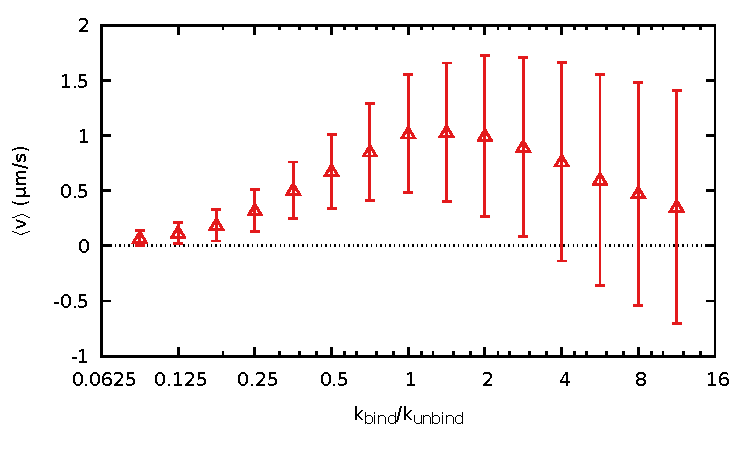
\includegraphics[width=0.45\textwidth,height=!]{v_k}
\caption{
\label{fig:v_k} 
Mean velocity of the motor relative to the actin filament $\langle v \rangle$ for varying $k_\text{bind}$.
The velocity decreases to $0$ for large discrepancies between binding and unbinding rate and reaches maximum when they are comparable.
}
\end{figure}


\section{Force -- velocity relation}
\label{sec:force-velocity}
In this section, we investigate the dependency of the mean velocity on an external load force $F_\text{load}$ applied to the motor parallel to the preferred direction, 
cf. figure~\ref{fig:ratchet setup}.
Figure~\ref{fig:F_v} shows the typical force -- mean velocity relations for various unbinding rates $k_\text{unbind}$, which mimics the dependency on ATP concentration.
Such a force-velocity relation was already presented in 2002 by Reimann \cite{reimann2002brownian}.
For small load forces, the response is very low. 
This is due to the interaction with an actin polymer, which provides an additional friction force to counter the load force. 
For larger forces the system looses its resilience and the contribution from the load will dominate. 
The larger the load, the more the velocity will approach the velocity of a non-interacting motor, $\langle v \rangle = \frac{1}{\gamma_\text{M}}F_\text{load}$.
Curves for higher ATP binding rates are closer to the curve for the completely unbound motor,
which means that the motor is more submissive to the external load.
\begin{figure}[t]
\centering
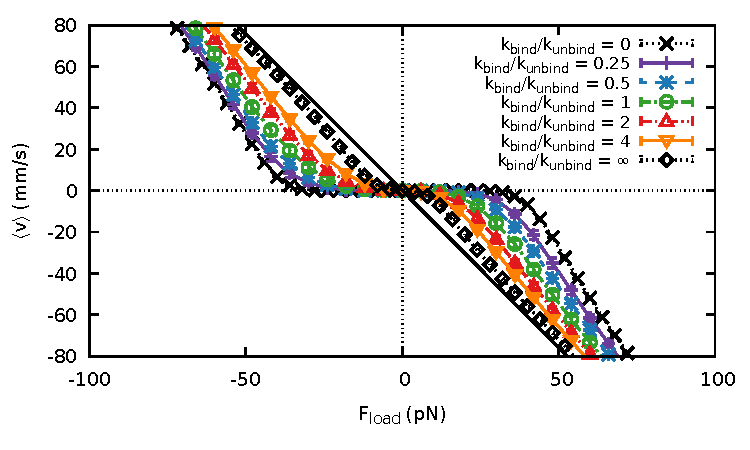
\includegraphics[width=0.45\textwidth,height=!]{F_v}
\caption{
\label{fig:F_v} 
Mean velocity $\langle v \rangle$ of the motor as a function of the load force $F_\text{load}$ for $c=0.3$ and for various binding rate $k_\text{bind}$.
Solid black line correspond to a situation where there will be no interaction with the actin filament, i.e. $\langle v \rangle = F_\text{load} / \gamma_\text{M}$. 
}
\end{figure}

A similar plot is shown in figure \ref{fig:F_v_heads}, where instead of varying binding rate $k_\text{bind}$ we look at motors with different numbers of heads $N$. Motors with only 1 head are very susceptible to external loads and the force from the ratchet offers little resistance. For 4 or 16 heads we see almost identical force-velocity relations. In section \ref{sec:efficiency}, however, we will see that these motors behave very differently regarding their energetics. 

\begin{figure}[t]
\centering
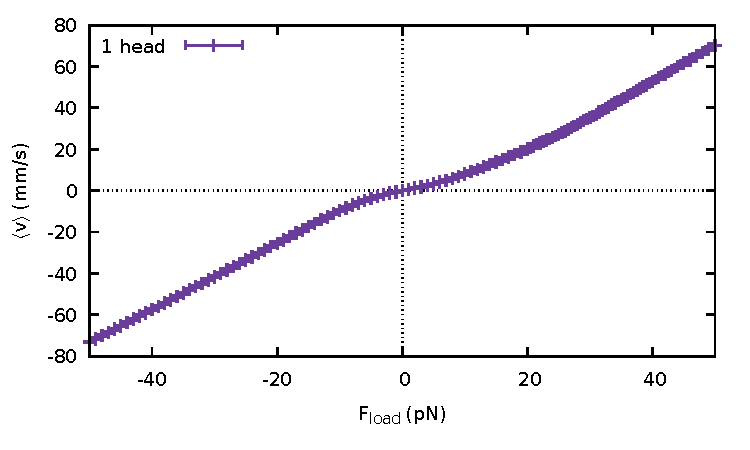
\includegraphics[width=0.45\textwidth,height=!]{F_v_heads}
\caption{
\label{fig:F_v_heads} 
Mean velocity $\langle v \rangle$ of the motor as a function of the load force $F_\text{load}$ for $c=0.3$ and for motors with different number of heads $N$.
Solid black line correspond to a non-interacting motor, i.e. $\langle v \rangle = F_\text{load} / \gamma_\text{M}$. 
}
\end{figure}

\subsection{Stall force}
From figure~\ref{fig:F_v} it is apparent, that when applying a force against the preferred direction of the motor, 
the motor first slows down until it stops before it reverses its direction. 
The force magnitude that is needed to stop the motor's movement relative to the actin filament is called the stall force $F_\text{stall}$,  
\[
\left\langle v ( F_\text{load} \equiv -F_\text{stall} ) \right\rangle = 0 .
\]
Figure~\ref{fig:F_v_zoom} shows the inset of figure~\ref{fig:F_v} for small negative loads. 
The intersections with the horizontal axis correspond to stall forces,  
while intersections of the curves with the vertical axis correspond to the mean velocities in figure \ref{fig:v_k}. 
We see that for small loads the mean velocity decreases linearly with increasing load. 
We observe that the slope of the force -- mean velocity relation increases with the binding rate $k_\text{bind}$. 
This is responsible for monotonous decrease of the stall force $F_\text{stall}$ with respect to the binding rate $k_\text{bind}$, see figure \ref{fig:k_Fstall}.
When the binding rate increases, so does the fraction of time in which the motor is less interacting with the actin filament. 
Hence, it will take on average a smaller load to halt a motor since the amplitude of its confining potential will be typically lower.
Ultimately, when the system is found only in the unbounded state the relative mean velocity is zero, $\langle v \rangle = 0$, as the system reached an equilibrium 
and thus the stall force reaches zero as well, $F_\text{stall} \to 0$.
%TODO Relate to power law => Maybe some analytics can help
\begin{figure}[t]
\centering
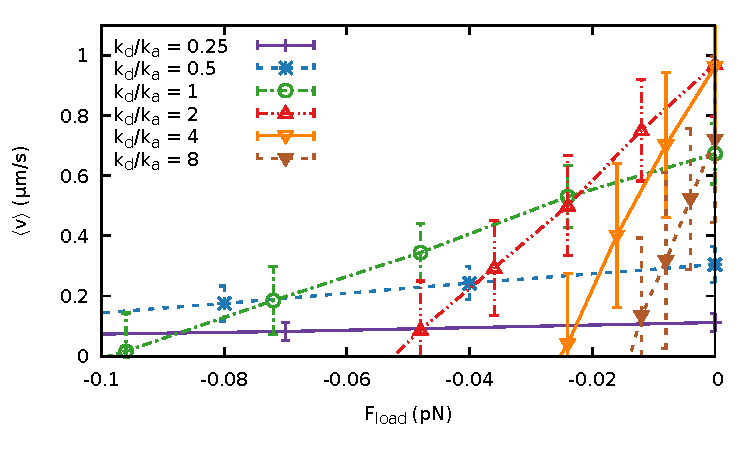
\includegraphics[width=0.45\textwidth,height=!]{F_v_zoom}
\caption{
\label{fig:F_v_zoom} 
Mean velocity of the motor $\langle v \rangle$ with a small load force $F_\text{load}$ applied in the direction opposing the movement for different binding rates $k_\text{bind}$.
Intersections with the $x$ axis correspond to stall forces $F_\text{stall}$ for given detach rates. 
We can see that with increasing $k_\text{bind}/k_\text{unbind}$ ratio the slope increases as well as the full curve shifts in the low force region, causing a persistent decrease in stall force.  
}
\end{figure}
\begin{figure}[t]
\centering
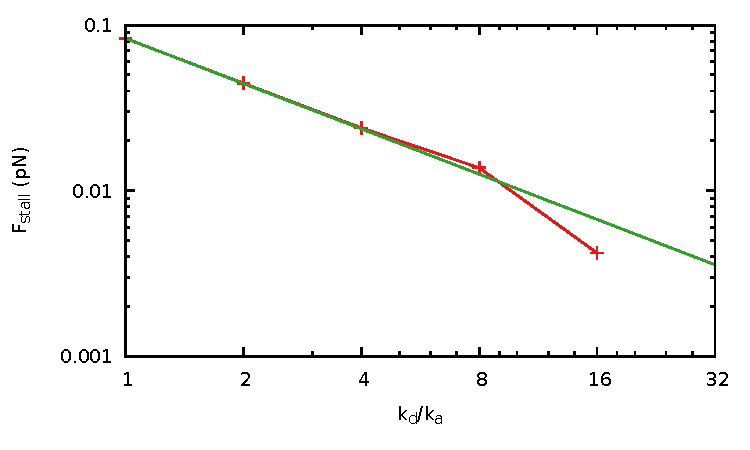
\includegraphics[width=0.45\textwidth,height=!]{k_Fstall}
\caption{
\label{fig:k_Fstall} 
Stall force $F_\text{stall}$ for different detach rates $k_\text{d}$.
We observe power-law decay $F_\text{stall} \propto k_\text{d}^{-\alpha}$ with exponent $\alpha = 1.002 \pm 0.014$. 
}
\end{figure}

\subsection{Velocity with respect to medium}
\label{sec:ind_velo}
Until now, we have investigated the relative velocity of the myosin and actin polymer, however this does not give us any information,
whether it is motor who is moving with respect to the medium or rather the actin polymer who is being pushed through the medium.
In order to find the dependency between individual velocities and relative velocity we start by taking the mean value of equations \eqref{eq:eom_M} and \eqref{eq:eom_A}
\begin{align}
\gamma_\text{M} \langle v_\text{M} \rangle &= \frac{ \langle \rmd x_\text{M} \rangle }{\rmd t} = \langle F_\text{r} \rangle + F_\text{load} , \label{eq:pre_velocity_M} \\
\gamma_\text{A} \langle v_\text{A} \rangle &= \frac{ \langle \rmd x_\text{A} \rangle }{\rmd t} = -\langle F_\text{r} \rangle , \label{eq:pre_velocity_A}
\end{align}
where $F_\text{r}$ denote ratchet force, 
$F_\text{r} = - \nabla_\text{M} V_t( x_\text{M} - x_\text{A} ) = \nabla_\text{A} V_t(x_\text{M} - x_\text{A} )$. 
Hence, the relative velocity in terms of the mean ratchet force is given by 
\begin{equation*}
\langle v \rangle 
= \langle v_\text{M} - v_\text{A} \rangle 
= \frac{\gamma_\text{A} + \gamma_\text{M}}{\gamma_\text{A} \gamma_\text{M}} \langle F_\text{r} \rangle + \frac{1}{\gamma_\text{M}} F_\text{load} ,
\end{equation*}
which yields to individual velocities in terms of the mean velocity and load 
\begin{align}
\langle v_\text{M} \rangle &= \frac{1}{ \gamma_\text{A} + \gamma_\text{M} } \left( \gamma_\text{A} \langle v \rangle + F_\text{load} \right) ,
\label{eq:velocity_M} \\
\langle v_\text{A} \rangle &= -\frac{1}{ \gamma_\text{A} + \gamma_\text{M} } \left( \gamma_\text{M} \langle v \rangle - F_\text{load} \right) .
\label{eq:velocity_A}
\end{align}
Note, that for the load equal the stall force, both velocities are equal and non-zero.
This is related to the fact that the full system is moving with respect to the liquid, as can be seen from the mean velocity of the geometric center 
\begin{multline*}
\langle v_\text{center} \rangle = \left\langle \frac{ v_\text{M} + v_\text{A} }{2} \right\rangle 
= \\
= \frac{ \gamma_\text{A} - \gamma_\text{M} }{ 2 ( \gamma_\text{A} + \gamma_\text{M} ) } \langle v \rangle + \frac{1}{ \gamma_\text{A} + \gamma_\text{M} } F_\text{load}
, 
\end{multline*}
which is proportional to both load and relative velocity and is zero only when $\langle v \rangle = - 2 F_\text{load} / ( \gamma_\text{A} - \gamma_\text{M} )$.

The dependency of individual velocities on the load is show in figure~\ref{fig:ind_v}, 
where we observe that for relatively small loads, the motor and actin filament are moving together, because the coupling by the ratchet interaction proves to be dominant. 
This can be explained by linear dependency of equations \eqref{eq:velocity_M} and \eqref{eq:velocity_A} on the load, 
along with the fact that for small loads the mean relative velocity is as well linear in the load, see figure~\ref{fig:F_v}. 
The inset of figure~\ref{fig:ind_v} then depicts the velocities for very small loads.
\begin{figure}[t]
\centering
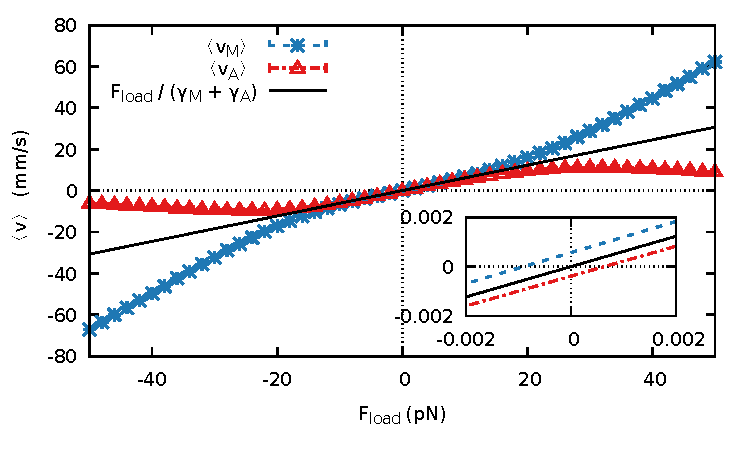
\includegraphics[width=0.45\textwidth,height=!]{individual_velocities}
\caption{
\label{fig:ind_v} 
Mean velocities of the motor and actin filament with respect to an inertial frame of reference for $k_d/k_a = 2$.
We observe that only the myosin is moving while the velocity of the dragged actin filament decreases as we increase the load on the myosin motor.
Inset: Zoomed to the linear regime around the origin.
}
\end{figure}

Since the load is only applied to the motor, for very high loads, the motor will start slipping over the ratchet potential along the actin filament. 
Consequently, the actin's mean velocity will stop increase and approaches zero for larger loads 
while the myosin's mean velocity go to $F_\text{load}/\gamma_\text{M}$ as can be seen in figure~\ref{fig:ind_v}. 
As well the relative velocity $\langle v \rangle$ will be equal to the motor's velocity $\langle v_M \rangle$ in that case, 
cf. equations~\eqref{eq:velocity_M} and~\eqref{eq:velocity_A}.
This is in good agreement with the figure~\ref{fig:F_v}.

\subsection{Ratchet force} 
One can interpret the nonlinear force-velocity relation for the myosin \eqref{eq:pre_velocity_M} as balance between the load, drag force and the force caused by the ratchet interaction, 
that intrinsically depends on the load. 
Without the ratchet interaction, the motion of the myosin would satisfy $ \gamma_\text{M}\langle v\rangle = F_\text{load}$. 
The discrepancy in this relation, up to a pre-factor, equals the mean force exerted via the flashing ratchet $\langle F_\text{r}\rangle$ 
\begin{equation*}
\frac{\gamma_\text{A}\gamma_\text{M}}{\gamma_\text{A} + \gamma_\text{M} } \left(\langle v \rangle - \frac{F_\text{load}}{\gamma_\text{M}}\right) = \langle F_\text{r} \rangle.
\end{equation*}
Note that this is the same as the distance between the force-velocity curves and the ratchet-free curve in figure \ref{fig:F_v}.
In figure \ref{fig:ratchet_force} we observe, 
that the response of the system for small loads is linear and independent of the rates and hence of the ATP concentration. 
In this regime the motor hardly moves along the filament and the load is almost completely countered by the mean ratchet force, i.e. it acts as a friction force.
The force generated by the ratchet interaction will reach a maximal value and eventually decay for larger external load forces. 
In section~\ref{sec:perturb} we will show that, as the load goes to infinity, the friction provided by the ratchet will go to zero as 
\begin{equation}
\left| \langle F_\text{r} \rangle_{F_\text{load}\rightarrow\infty} \right| \asymp \frac{1}{F_\text{load}} , 
\label{eq:ratchet_vs_load}
\end{equation} 
which is shown in figure \ref{fig:ratchet_force_decay}. 
\begin{figure}[t]
\centering
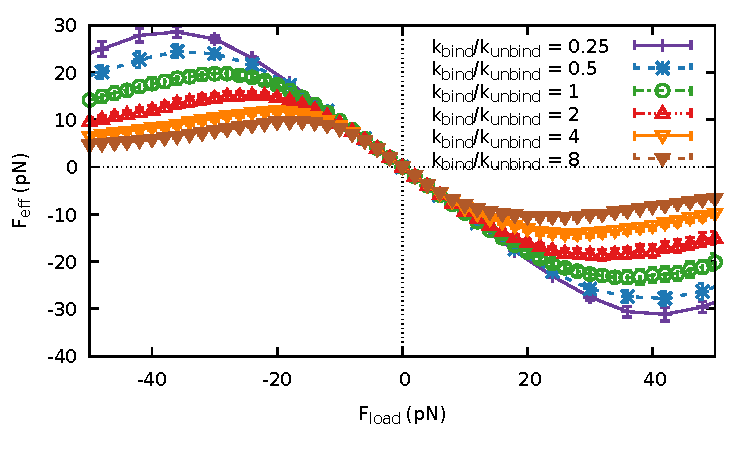
\includegraphics[width=0.45\textwidth,height=!]{ratchet_force}
\caption{
\label{fig:ratchet_force}
Effective friction force from the ratchet interaction depending on the load force on the motor.
}
\end{figure}
\begin{figure}[t]
\centering
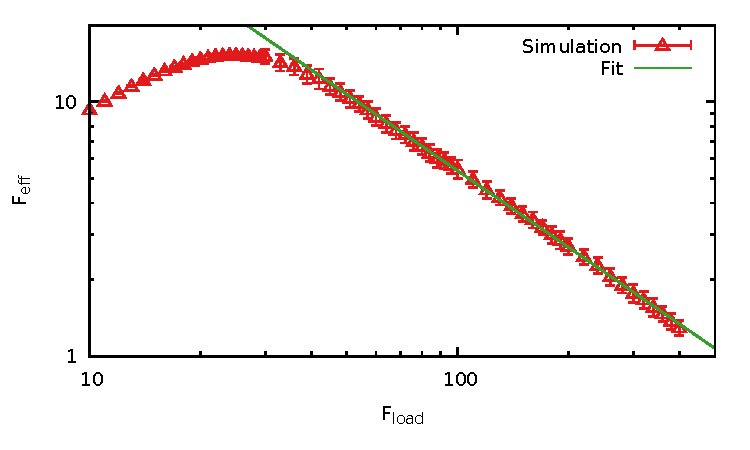
\includegraphics[width=0.45\textwidth,height=!]{ratchet_force_decay}
\caption{
\label{fig:ratchet_force_decay}
The ratchet force, depending on the load, is shown in a logarithmic plot. 
We can see that the ratchet force asymptotically decays according to the power law $F_\text{eff} \propto F_\text{load}^{-\alpha}$, 
with exponent determined from the fit to be $\alpha = 0.9990 \pm 0.0047$, 
which is in good agreement with the theoretical prediction \eqref{eq:ratchet_vs_load}.
}
\end{figure}

\subsection{Tension in the motor}

The force-velocity relation can also be exploited to derive the tension in the motor. 
Since both the load and ratchet force are directly applied to the motor, the tension can be derived from equations \eqref{eq:pre_velocity_M}, \eqref{eq:pre_velocity_A}, \eqref{eq:velocity_M} and \eqref{eq:velocity_A}.
\begin{align}
\langle F_\text{r} \rangle - F_\text{load} 
&= - \gamma_\text{M} \langle v_\text{M} \rangle - 2\gamma_\text{A} \langle v_\text{A} \rangle \nonumber \\
&= \frac{\gamma_\text{A}\gamma_\text{M}}{\gamma_\text{A}+\gamma_\text{M}}\langle v\rangle - \left(1 + \frac{\gamma_\text{A}}{\gamma_\text{A}+\gamma_\text{M}} \right) F_\text{load}
\label{eq:tension}
\end{align}

A similar analysis can be made for the setup in section \ref{sec:load_on_fil}. 
There, the motor is in the middle of this symmetric setup and will not move on average. 
The mean velocities of the actin filaments and motor are given by
\begin{align*}
\langle v_{\text{A}_1} \rangle &= \frac{1}{\gamma_\text{A} } \left( F_\text{load} - \langle F_\text{r1} \rangle \right) \\
\langle v_\text{M} \rangle &= \frac{1}{\gamma_\text{M} } \left( \langle F_\text{r1} \rangle + \langle F_\text{r2} \rangle \right)\\
\langle v_{\text{A}_2} \rangle &= \frac{1}{ \gamma_\text{A} } \left( - F_\text{load} - \langle F_\text{r2} \rangle \right) 
\end{align*}
where ${\text{A}_1}$ and ${\text{A}_2}$ denote the two different actin filaments and $F_\text{r1}$ and $F_\text{r2}$ are the ratchet forces between the motor and respectively filament ${\text{A}_1}$ and ${\text{A}_2}$. 

Note that the mean velocity of the motor is proportional to the mean center of mass velocity of both actin filaments. 
\begin{equation}
\langle v_\text{M} \rangle = \frac{\gamma_\text{A}}{\gamma_\text{M}} \left(\langle v_{\text{A}_1} \rangle + \langle v_{\text{A}_2} \rangle \right) 
\label{eq:tug_F_motor}
\end{equation}
Because of the anti-parallel alignment of the filaments, $F_{r1}$ and $F_{r2}$ are equal but opposite on average. 
Therefore the motor will not experience any mean displacement.  

Although the motor doesn't experience an external load and it will not have a net force on average, there will be a tension on the motor due to interaction with both actin filaments. This tension is given by
\begin{equation*}
\langle F_\text{r1}\rangle - \langle F_\text{r2}\rangle = -\gamma_\text{A}\left(\langle v_{\text{A}_1}\rangle - \langle v_{\text{A}_2}\rangle \right) - 2F_\text{load}
\end{equation*}
The tension in the motor is shown in figure \ref{fig:tug_F}, where it is compared to the tension when the load is applied on the motor instead of the filaments, given by \eqref{eq:tension}. 

\begin{figure}[t]
\centering
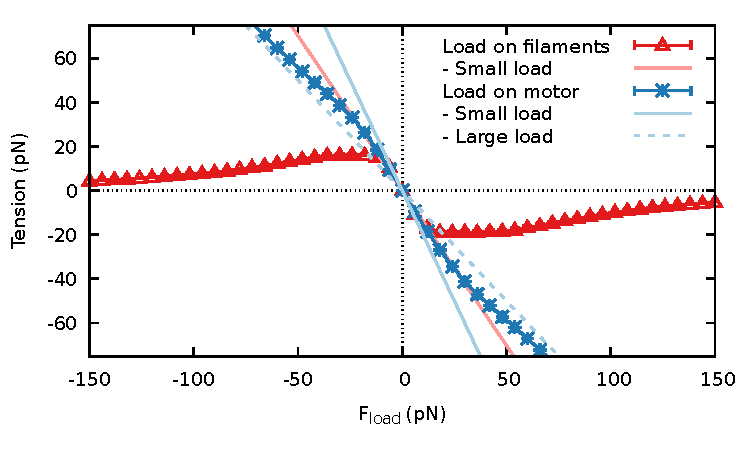
\includegraphics[width=0.45\textwidth,height=!]{tug_F}
\caption{
\label{fig:tug_F}
Tension in the motor, comparison between setup \ref{sec:load_on_fil} with two loaded filaments and the simple setup with one filament and a load on the motor. 
The tension for small loads follows the same trend, whereas for large loads the tension on the motor differs. 
This because, only in the simple setup, the load is directly applied to the motor resulting in an asymptotic tension. %TODO fix y label
}
\end{figure}

For small loads, the tension in both cases is equal to twice the load force. As we have seen in section \ref{sec:force-velocity}, the ratchet force tends to completely oppose the load. 
Therefore, the loads are transmitted from the filaments to the motor.
For larger load, the tensions in the different setups will differ. The motor and filaments start to slip, as in section \ref{sec:ind_velo}. 
Consequently, the mean ratchet force decreases and the increase in tension diminishes.
The difference in the two setups lies in the fact that, in the simple setup, the load is applied directly to the motor. As the ratchet force vanishes for large load, a residual tension from the load remains.
In the other setup, the tension on the motor is completely due to the forces from the ratchet interaction with the two filaments. For large loads this tension goes to zero as the mean ratchet forces go to zero. 

The empirical velocity of the motor, in setup \ref{sec:load_on_fil}, is plotted in figure \ref{fig:tug_F_motor}. 

\begin{figure}[t]
\centering
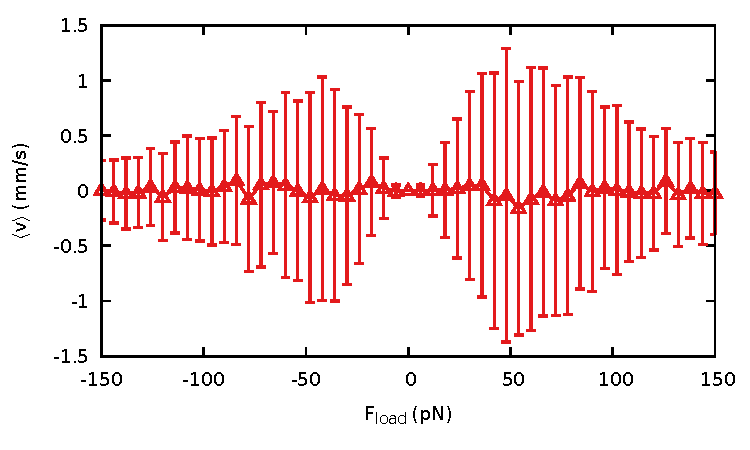
\includegraphics[width=0.45\textwidth,height=!]{tug_F_motor}
\caption{
\label{fig:tug_F_motor}
Mean velocity of frustrated motor in between the two filaments under load. The variance of the motor's velocity grows as the load increases. For even larger loads the motor and filaments start slipping and the variance decreases again.
}
\end{figure}

The variance of the motor velocity seems to behave similarly to the tension on the motor in figure \ref{fig:tug_F}. While the mean velocity stays close to zero, the variance increases as the tension builds up in the motor. As the motor begins to slip over the filaments, the variance appears to decrease again.


\subsection{Mechanosensing}
\label{sec:mechanosensing}
In this section we will look at the force that the motor generates and transfers to the filaments in the setup, sketched in figure \ref{fig:tug}. 
The mean force, which is measured through the extension of the springs, is plotted in figure \ref{fig:tug_k} for different stiffnesses $k$ that represent the surrounding network.
\begin{figure}[t]
\centering
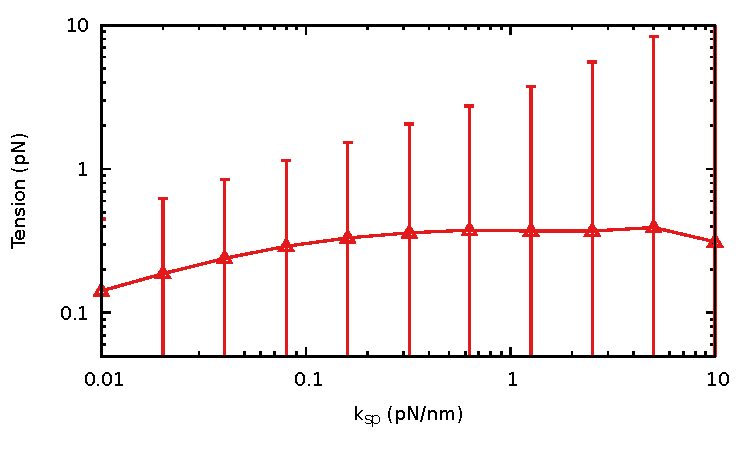
\includegraphics[width=0.45\textwidth,height=!]{tug_k}
\caption{
\label{fig:tug_k}
Mean force $F_\text{fil}$ generated by the motor on one of the filaments for varying spring stiffness $k_\text{sp}$.
Lower stiffness enables the polymers to find a local minimum of the ratchet potential more easily, 
thus the exerted force is lower as the contribution of ratchet potential is minimized. 
On the other hand, high stiffness leads to saturation of the exerted force as the main contribution is given by ratchet potential. 
}
\end{figure}
The force with which the motor pulls on the filament depends strongly on this elasticity $k$ and saturates for large $k$. 
This suggests that the motor is not only able to sense external forces, but also its environment's mechanical properties.
Similar results were obtained for different motor models with load dependent chemical rates \cite{stam2015isoforms,albert2014stochastic}. 
However, the models used in those studies exhibit rates the depend on the strain or tension in the myosin motor. 
In our study, we show that similar behaviour also occurs in a simple flashing ratchet with constant chemical rates. 
It is important to include the fluctuations in this stochastic model to preserve the mechanosensing feature. In mean field models, where the force-velocity relation would be is implemented such that the velocity of the motor depends deterministically on the load, the motor will essentially stall in this given setup and cease to exert a force on the filaments. 
Therefore mechanosensing will not occur spontaneously in those models.

\section{First law of thermodynamics}
\label{sec:energie}
Before we discuss an efficiency of the myosin in various setups, 
we need to introduce the basic notion of energy, heat and work. 
We start our discussion from the energy balance on the level of individual trajectories \cite{Pesek2013},
which can be symbolically summarized as 
\begin{equation}
\rmd E = \dbar {\mathcal Q}_\text{M}^\text{hb} + \dbar {\mathcal Q}_\text{A}^\text{hb} + \dbar {\mathcal W}^\text{ext}_\text{M} + \dbar {\mathcal Q}^\text{chem}, 
\label{eq:energy_balance}
\end{equation}
where the energy of the full system consists of the interaction ratchet potential \eqref{eq:ratchet_interaction}
and the energy stored in ATP (and its products), 
\begin{equation}
E( x_\text{M}, x_\text{A}, \{ \zeta_i \}) = V_t( x_\text{M} - x_\text{A} ) + \Delta E \sum\limits_{i=0}^{N-1} \chi( \zeta_i = c ) ,
\label{eq:internal_energy}
\end{equation}
where $\Delta E$ represents the actual internal energy stored by a single ATP and $\chi$ is a characteristic function\footnote{
$\chi(\text{condition}) = 1$ if condition is fulfilled otherwise $0$.
}.

The energy of the system is subjected to the change driven by the interaction with the environment, 
which in case of the overdamped diffusion represents a heath bath 
and thus every interaction is associated with a heat exchange \cite{Pesek2013}
\begin{align}
{\mathcal Q}_\text{M}^\text{hb} 
&= \int \rmd x_\text{M} \circ \left[ - \gamma_\text{M} \frac{\rmd x_\text{M} }{\rmd t} + \sqrt{ 2 k_B T \gamma_\text{M} } \, \frac{ \rmd W_\text{M} }{ \rmd t } \right] , 
\label{eq:heat_hb_M} \\
{\mathcal Q}_\text{A}^\text{hb} 
&= \int \rmd x_\text{A} \circ \left[ - \gamma_\text{A} \frac{\rmd x_\text{A} }{\rmd t} + \sqrt{ 2 k_B T \gamma_\text{A} } \, \frac{ \rmd W_\text{A} }{ \rmd t } \right] ,
\label{eq:heat_hb_A}
\end{align} 
where the first term is the dissipation of the energy due to the friction and the second is the energy gained by the thermal activity of the environment. 
Note that those integrals are evaluated in the Stratonovich sense.
The energy is also changed by the work of the external load 
\begin{equation}
{\mathcal W}^\text{ext}_\text{M} = \int \rmd x_\text{M} \circ F_\text{load} = \Delta x_\text{M} F_\text{load}, 
\label{eq:work_load}
\end{equation}
where we used the fact that the external load $F_\text{load}$ is constant. 

The last term in the energy balance \eqref{eq:energy_balance} is the contribution from the chemical cycle. 
The chemical cycle, in the most basic form \cite{}, consists of binding an ATP, it's hydrolyses, release of phosphor and finally release of ADP, %TODO
the first part provides a chemical energy to the system stored in ATP and ADP while the later part is associated with dissipation of the remaining energy to surroundings. 
Thus the total chemical energy consists of two parts ${\mathcal Q}^\text{chem} = {\mathcal Q}^\text{chem}_\text{in} + {\mathcal Q}^\text{chem}_\text{out}$,
\begin{align}
{\mathcal Q}_\text{in}^\text{chem} 
&= \sum_{t_\text{unbind} \leq t_\text{fin} } \left[ \Delta E + (c-1) V_r(x_{t_\text{unbind}}) \right] , 
\label{eq:q_in} \\
{\mathcal Q}_\text{out}^\text{chem} 
&= -\sum_{t_\text{bind} \leq t_\text{fin} } \left[ \Delta E + (c-1) V_r(x_{t_\text{bind}}) \right] 
\label{eq:q_out}
\end{align}
where we sum over all jump times $t_\text{bind}$($t_\text{unbind}$) in the given ``direction''. 
$t_\text{fin}$ denotes the duration of the process. 

\subsection{Load on the motor}
If we restrict the discussion only to the simplest setup, i.e. single loaded myosin with single actin,  
and we use the equation of motion \eqref{eq:eom_M}, 
the heat exchange with the surrounding \eqref{eq:heat_hb_M} can be rewritten as 
\begin{multline*}
{\mathcal Q}_\text{M}^\text{hb} 
= \int \rmd x_\text{M} \circ \left[ \nabla_\text{M} V_t(x_\text{M} - x_\text{A} ) - F_\text{load} \right] 
\\
= \int \rmd x_\text{M} \circ \nabla V_t(x_\text{M} - x_\text{A} ) - {\mathcal W}_\text{M}^\text{ext} ,
\end{multline*}
where $\nabla V_t$ denotes the derivative with respect to the argument. 
Similarly for the heat dissipated by actin's interaction with the environment we get 
\begin{multline*}
{\mathcal Q}_\text{A}^\text{hb} 
= \int \rmd x_\text{A} \circ \nabla_\text{A} V_t(x_\text{M} - x_\text{A} )
\\
= - \int \rmd x_\text{A} \circ \nabla V_t(x_\text{M} - x_\text{A} ) ,
\end{multline*}
thus the heat dissipated to heath bath can be expressed in terms of the work done by the ratchet potential and external load. 
Consequently, the total energy balance equation \eqref{eq:energy_balance} simplifies to 
\[
\rmd E 
= \rmd x_\text{M} \circ \nabla_\text{M} V_t  
+ \rmd x_\text{A} \circ \nabla_\text{A} V_t  
+ {\mathcal Q}_\text{in}^\text{chem}
+ {\mathcal Q}_\text{out}^\text{chem} , 
\]
which does not explicitly depend on the load $F_\text{load}$. 


\subsection{Heat fluxes}
At last, note that the internal energy of the system \eqref{eq:internal_energy} is bounded.
Hence, if we interpret the energy balance equation \eqref{eq:energy_balance} in terms of mean dissipation rates defined as 
\begin{equation}
q = \lim_{\Delta t \to \infty} \frac{1}{\Delta t} \left\langle {\mathcal Q}(\Delta t) \right\rangle ,
\label{eq:heat_flux}
\end{equation}
we obtain en equation representing the conservation of fluxes 
\begin{equation}
0 = q_\text{M}^\text{hb} + q_\text{A}^\text{hb} + w^\text{ext}_\text{M} + q^\text{chem} 
\label{eq:heat_flux_balance}
\end{equation}
for arbitrary initial condition. 
Such equality is trivially true for arbitrarily small time when the initial condition corresponds the steady state. 


\subsection{Tug of war} 
In section \ref{sec:ratchet} we introduced two alternative models more suitable for capturing the behavior of myosin inside the polymer network known as actomyosin cortex.

\subsubsection{Force on filaments}
In the first model, see paragraph~\ref{sec:load_on_fil} and figure~\ref{fig:tug_F_illustration},
the myosin is attached between two polymers on which the load is applied, 
hence the energy balance \eqref{eq:energy_balance} is modified to  
\begin{multline}
\rmd E = \dbar {\mathcal Q}_\text{M}^\text{hb} + \dbar {\mathcal Q}_{\text{A}_1}^\text{hb} + \dbar {\mathcal Q}_{\text{A}_2}^\text{hb} 
\\
+ \dbar {\mathcal W}^\text{ext}_{\text{A}_1} + \dbar {\mathcal W}^\text{ext}_{\text{A}_2} + \dbar {\mathcal Q}^\text{chem}, 
\label{eq:energy_balance_two_filaments}
\end{multline}
where the energy now contains contributions from both polymers
\begin{multline*}
E( x_\text{M}, x_{\text{A}_1}, x_{\text{A}_2}, \{ \zeta_i \}) 
= V_t( x_\text{M} - x_{\text{A}_1} ) 
\\
+ V_t( x_{\text{A}_2} - x_\text{M} ) 
+ \Delta E \sum\limits_{i=0}^{N-1} \chi( \zeta_i = c ) .
\end{multline*}
Note, that the last sum is over all heads of the motor, $N = N_{\text{A}_1} + N_{\text{A}_2}$.
Contributions from the heat exchange with environment \eqref{eq:heat_hb_A} remains the same, even though in this case we have two contributions from both filaments
\begin{align*}
{\mathcal Q}_{\text{A}_1}^\text{hb} 
&= \int \rmd x_{\text{A}_1} \circ \left[ - \gamma_\text{A} \frac{\rmd x_{\text{A}_1} }{\rmd t} + \sqrt{ 2 k_B T \gamma_\text{A} } \, \frac{ \rmd W_{\text{A}_1} }{ \rmd t } \right] , \\ 
{\mathcal Q}_{\text{A}_2}^\text{hb} 
&= \int \rmd x_{\text{A}_2} \circ \left[ - \gamma_\text{A} \frac{\rmd x_{\text{A}_2} }{\rmd t} + \sqrt{ 2 k_B T \gamma_\text{A} } \, \frac{ \rmd W_{\text{A}_2} }{ \rmd t } \right] ,
\end{align*}
and the external load is now not applied on the motor but on each actin polymer.
Thus the equation \eqref{eq:work_load} is replaced by 
\begin{align*}
{\mathcal W}^\text{ext}_{\text{A}_1} &= \int \rmd x_{\text{A}_1} \circ F_\text{load} = \Delta x_{\text{A}_1} F_\text{load}, 
\\
{\mathcal W}^\text{ext}_{\text{A}_2} &= - \int \rmd x_{\text{A}_2} \circ F_\text{load} = - \Delta x_{\text{A}_2} F_\text{load}. 
\end{align*}

Note, that the interpretation of the energy balance \eqref{eq:energy_balance_two_filaments} in terms of the heat fluxes \eqref{eq:heat_flux}
while following the same arguments as for \eqref{eq:heat_flux_balance} is possible and leads to   
\[
0 = q_\text{M}^\text{hb} + q_{\text{A}_1}^\text{hb} + q_{\text{A}_2}^\text{hb} + w^\text{ext}_{\text{A}_1} + w^\text{ext}_{\text{A}_2} + q^\text{chem} .
\]

\subsubsection{Elastic environment}
The second model, described in paragraph \ref{sec:environment} and depicted in figure \ref{fig:tug}, 
modifies the energy balance \eqref{eq:energy_balance}, resp. \eqref{eq:energy_balance_two_filaments}, even further
\begin{equation*}
\rmd E = \dbar {\mathcal Q}_\text{M}^\text{hb} + \dbar {\mathcal Q}_{\text{A}_1}^\text{hb} + \dbar {\mathcal Q}_{\text{A}_2}^\text{hb} + \dbar {\mathcal Q}^\text{chem}, 
\end{equation*}
as there is no external load but all the accumulated energy is now stored in harmonic potentials 
\begin{multline*}
E( x_\text{M}, x_{\text{A}_1}, x_{\text{A}_2}, \{ \zeta_i \}) 
= V_t( x_\text{M} - x_{\text{A}_1} ) 
+ V_t( x_{\text{A}_2} - x_\text{M} ) 
\\
+ \frac{1}{2} k \left[ x_{\text{A}_1} - x_{\text{A}_1}(0) \right]^2 
+ \frac{1}{2} k \left[ x_{\text{A}_2} - x_{\text{A}_2}(0) \right]^2 
\\
+ \Delta E \sum\limits_{i=0}^{N-1} \chi( \zeta_i = c ) .
\end{multline*}
Contrary to the previous setup, the total energy of the system is no longer bound and hence the heat fluxes \eqref{eq:heat_flux} are only balanced in the steady state. 

\section{Chemical efficiency} 
\label{sec:efficiency}
In previous years, a lot of effort was directed towards the assessment of the efficiency of molecular motors \cite{}. %TODO 
Unfortunately, main focus of these works was biased towards the transport properties of the aforementioned motors. 
However myosin II main role is in generating of the tension in the cytoskeletal network \cite{}. %TODO

Efficiency, in general, relate a ``useful'' output with the input.
As the ``usefulness'' heavily depends on the setup, there is a plethora of possible choices.
Here we discuss one common choice and one choice, to the best knowledge of authors, previously not discussed in the leturature. 
The first definition of the chemical efficiency, well discussed in the literature \cite{}, is related to the transport properties of molecular motors. 
The second definition of the chemical efficiency captures the speed of the tension generation in networks, which typically contain a myosin~II. 

\subsection{Transport efficiency} 
As we have stated, the first efficiency we discuss is related to transport properties. 
Namely, we identify the heat dissipated to the environment by the motor alone as the output work 
\[
{\mathcal W}^\text{out}_\text{M} = - {\mathcal Q}^\text{hb}_\text{M} 
\] 
and chemical work $\mathcal Q^\text{chem}$ and the work done by the load $\mathcal W^\text{ext}_\text{M}$.
Hence the transport efficiency can be defined as 
\[
\eta_\text{tr} = \frac{ \left\langle {\mathcal W}^\text{out}_\text{M} \right\rangle }{ \left\langle {\mathcal Q}^\text{chem} \right\rangle + \left\langle {\mathcal W}^\text{ext}_\text{M} \right\rangle } .
\]
Note, that for large load ($F_\text{load} \to \infty$) such efficiency approaches $\eta_\text{tr} \to 1$, 
while for no load $F_\text{load} = 0$ it captures how much of the chemical energy get dissipated by the motor's motion  
\[
\eta_\text{tr}( F_\text{load} = 0 ) = \frac{ \left\langle \int \rmd x_\text{M} \circ \left[ - \nabla_M V_t \right] \right\rangle }{ \left\langle {\mathcal Q}^\text{chem} \right\rangle } ,
\]
i.e. how much of the chemical energy provided to the system is dissipated by the motor and not by the polymer. 


\subsection{Chemical cycle efficiency} %TODO 
Alternative approach it to identify as the ``useful'' is ratio the chemical energy supplied by ATP which is transformed to other forms of energy, 
i.e. either is dissipated by myosin and actin through they diffusion or is stored in the interaction potential and thus increase the tension in the system. 
This consideration leads to chemical cycle efficiency defined as 
\begin{equation}
\eta_\text{chem} = \frac{\langle\mathcal Q^\text{chem}_\text{in}\rangle+\langle\mathcal Q^\text{chem}_\text{out}\rangle}{\langle\mathcal Q^\text{chem}_\text{in}\rangle} .
\label{eq:efficiency}
\end{equation}

\subsubsection{Simple setup}
For a system in a simple setup with four heads, we investigate the dependency of such chemical efficiency on the load, see figure~\ref{fig:chem}.
We observe that the chemical efficiency has two local maximums. 
We will later show that these two maximums correspond to a frustrated system, 
where the load is close to the point where it is able to overpower any forces induced by the ratchet potential. 
Another observation, which we will discuss in depth later, is that the efficiency reaches a negative value, 
which we interpret as a situation where the work done by the load $F_\text{load}$ is converted back to chemical energy. 
\begin{figure}[t]
\centering
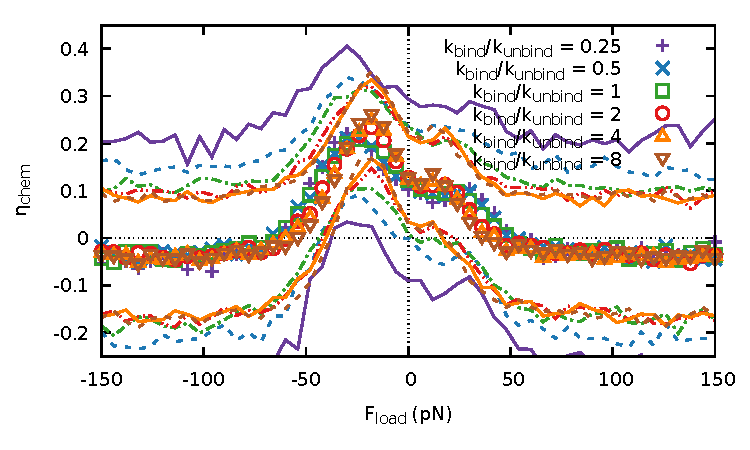
\includegraphics[width=0.45\textwidth,height=!]{chemical_cycle}
\caption{
\label{fig:chem}
Chemical efficiency $\eta$ as a function of load force $F_\text{load}$.
Solid lines are plotted at the level of $1\sigma$. 
By increasing the $k_d/k_a$ ratio the local maximums of chemical efficiencies are getting closer origin,
and their fluctuations decrease. 
}
\end{figure}

In order to properly understand these features, 
we try evaluate the chemical efficiency \eqref{eq:efficiency} in a steady state. 
We start by evaluating the mean heat \eqref{eq:q_in} and \eqref{eq:q_out} produced over a time interval of length $\Delta t$ 
by transitions of a single head $i$ displaced by $i d$  
\begin{gather*}
\begin{multlined}[b][.42\textwidth]
\langle \mathcal Q^\text{chem}_\text{in}(i) \rangle 
= \Delta t \, k_\text{unbind} 
\\ \times 
\!\!\!\! \sum\limits_{\{\zeta_j\} : \zeta_i = 1 } \!\!\!\! \rho(\{ \zeta_j \} ) 
\left[ \Delta E - (1-c) \left\langle V_r(x - i \, d ) \middle| \{ \zeta_j \} \right\rangle \right] 
\end{multlined}
%\label{eq:mean_q_in} 
\\
\begin{multlined}[b][.42\textwidth]
\langle \mathcal Q^\text{chem}_\text{out}(i) \rangle 
= - \Delta t \, k_\text{bind} 
\\ \times 
\!\!\!\! \sum\limits_{\{\zeta_j\} : \zeta_i = c } \!\!\!\! \rho(\{ \zeta_j \} ) 
\left[ \Delta E - (1-c) \left\langle V_r(x - i \, d ) \middle| \{ \zeta_j \} \right\rangle \right] 
\end{multlined}
%\label{eq:mean_q_out}
\end{gather*}
where $\langle V | X \rangle$ is the steady state conditional mean value with respect to the fixed internal state $X$ 
and $\rho(X) \in [0,1]$ denotes the probability of the occupation of the corresponding internal state $X$ in a steady state, 
which does not depend on the position due to the independence of the positional independence of its internal dynamics~\eqref{eq:transition}. 
Moreover, due to the independence of individual heads the probability occupation of a given internal state can be written as 
\[
\rho( \{ \zeta_i \} ) = \prod_{i=0}^{N-1} \rho_1( \zeta_i ), 
\]  
where 
\[
\rho_1(\zeta) = \begin{cases} 
\frac{ k_\text{bind} }{ k_\text{bind} + k_\text{unbind} } & \zeta = 1 , \\
\frac{ k_\text{unbind} }{ k_\text{bind} + k_\text{unbind} } & \zeta = c . 
\end{cases} 
\]

Another consequence of the independence of the time evolution of individual heads is, 
that we can express the total mean heats produced in chemical cycle as a sum of contributions from individual heads
\begin{align*}
\langle \mathcal Q_\text{in}^\text{chem} \rangle 
=& \sum\limits_{i=0}^{N-1} \left\langle \mathcal Q_\text{in}^\text{chem}(i) \right\rangle 
= \Delta t \frac{ k_\text{bind} k_\text{unbind} }{ k_\text{bind} + k_\text{unbind} } 
\\ &\times
\left[ N \, \Delta E 
- (1-c) \sum\limits_{i=0}^{N-1} \left\langle V_r(x - i d ) \middle| \zeta_i = 1 \right\rangle 
\right] ,  
\\
\langle \mathcal Q^\text{chem}_\text{out} \rangle 
=& \sum\limits_{i=0}^{N-1} \left\langle \mathcal Q_\text{out}^\text{chem}(i) \right\rangle 
= - \Delta t \frac{ k_\text{bind} k_\text{unbind} }{ k_\text{bind} + k_\text{unbind} } 
\\ &\times
\left[ N \, \Delta E 
- (1-c) \sum\limits_{i=0}^{N-1} \left\langle V_r(x - i d ) \middle| \zeta_i = c \right\rangle  
\right] , 
\end{align*}
which leads to a more explicit expression for the efficiency \eqref{eq:efficiency} 
\begin{multline*}
\eta_\text{chem} = \frac{1-c}{N}
\\ \times
\sum\limits_{i=0}^{N-1} \frac{ \left\langle V_r(x-id) \middle| \zeta_i = c \right\rangle - \left\langle V_r( x -id ) \middle| \zeta_i = 1 \right\rangle }
{ \Delta E - \frac{1-c}{N} \sum\limits_{j=0}^{N-1} \left\langle V_r(x-jd) \middle| \zeta_j = 1 \right\rangle } 
. 
\end{multline*}
We can further introduce an average probability density of a single head 
\begin{equation}
\bar{\rho}(x,\zeta) = \frac{1}{N} \sum\limits_{i=0}^{N-1} \sum\limits_{ \{ \zeta_j \} : \zeta_i = \zeta } \rho( x + i d, \{ \zeta_j \} ) ,
\label{eq:eff_distribution}
\end{equation}
which allow us to further simplify the expression for the chemical efficiency to 
\begin{equation}
\eta_\text{chem} = (1-c)
\frac{ \left\langle V_r(x) \middle| \zeta = c \right\rangle_{\bar{\rho}} - \left\langle V_r(x) \middle| \zeta = 1 \right\rangle_{\bar{\rho}} }
{ \Delta E - (1-c) \left\langle V_r(x) \middle| \zeta = 1 \right\rangle_{\bar{\rho}} } 
. 
\label{eq:eta}
\end{equation}
We can see that the numerator is given by the average difference between mean potentials in ATP attached and detached states over all heads. 
As the potential is known in our model, the only missing information is thus the steady state distribution 
or to be more precise the average steady state density for a single head \eqref{eq:eff_distribution}.  
These distributions are empirically obtained by collecting the positions of the heads over all times that the head was in the ATP bound/unbound state 
and are shown in figure~\ref{fig:pos_distr} for different load forces. 
\begin{figure}[t]
\centering
\subfigure[ATP unbound state]{ 
\centering
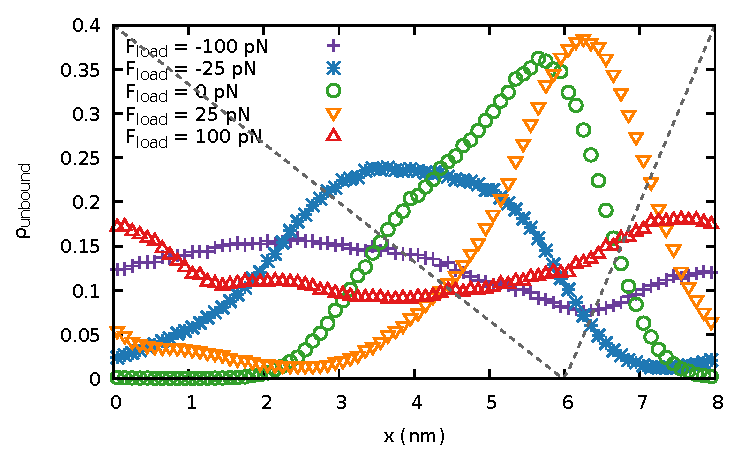
\includegraphics[width=.45\textwidth,height=!]{pos_distr_a_F}
}
\\
\subfigure[ATP bound state]{
\centering
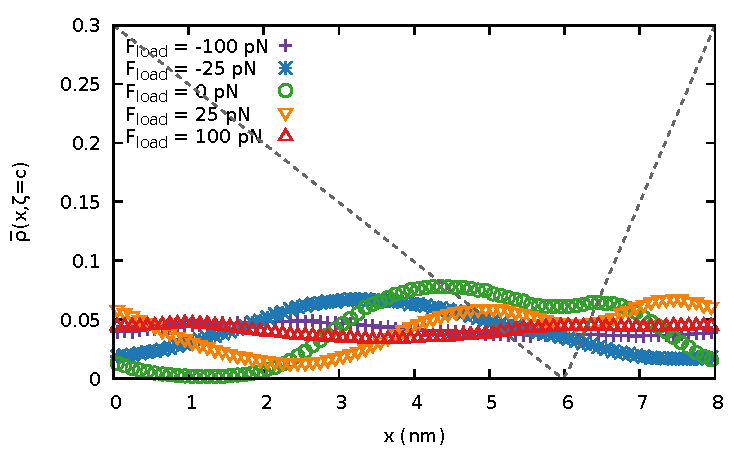
\includegraphics[width=.45\textwidth,height=!]{pos_distr_d_F}
}
\caption{
\label{fig:pos_distr}
Spatial distributions $\rho$ of individual heads of the motor with respect to the ratchet potential (denoted by dashed black line) for different load forces $F_\text{load}$.
The spatial distribution is taken as the average over all heads at the given motor in a given internal state.
We observe that heads in the attachable state follow the potential closely while those in the detached state do not. 
Also by increasing the external load, all distributions universally become flat. 
}
\end{figure}

The difference between the average distribution \eqref{eq:eff_distribution} in the ATP bound state and ATP unbound state is directly translated to the mean heat flux \eqref{eq:heat_flux} out of the chemical system
\begin{multline*}
q_\text{in}^\text{chem} + q_\text{out}^\text{chem} 
= (1-c) \frac{ k_\text{bind} k_\text{unbind} }{ k_\text{bind} + k_\text{unbind} } 
\\ \times
\left[ \left\langle V_r(x) \middle| \zeta = c \right\rangle_{\bar{\rho}} - \left\langle V_r(x) \middle| \zeta = 1 \right\rangle_{\bar{\rho}} \right] .
\end{multline*} 
This is summarized in the figure~\ref{fig:chem_energy_distr}, 
where we show the spatial dependency of the given heat flux.
We can see a major contribution from the tails where the difference in the average densities is weighted by potential maximum.
\begin{figure}[t]
\centering
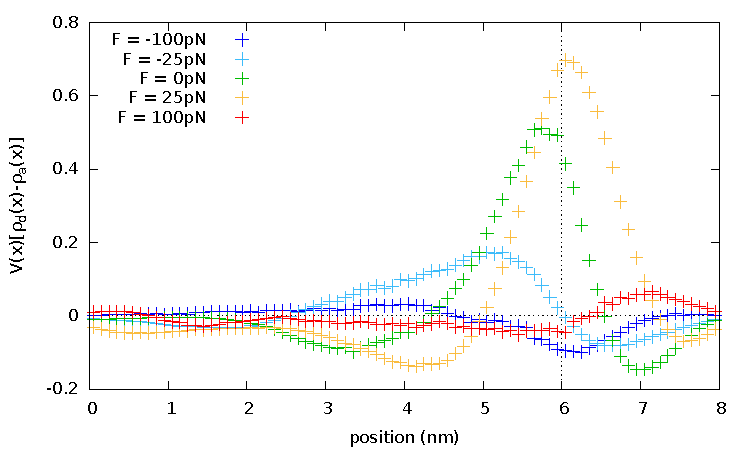
\includegraphics[width=0.45\textwidth,height=!]{chem_energy_distr_all_F}
\caption{
\label{fig:chem_energy_distr}
Space resolved denominator of the efficiency \eqref{eq:eta} for various load forces $F_\text{load}$. %TODO
We observe that the optimal output is achieved when there is the biggest discrepancy between spatial distributions, compare with figure~\ref{fig:pos_distr} and \ref{fig:chem}. 
}
\end{figure}

In the case without external load, $F_\text{load}=0$, 
the maximum of the distribution, see fig.~\ref{fig:pos_distr}, is close to the minimum of the potential,  
where the discrepancy in the position comes from the averaging over multiple heads with a fixed distance between them, 
which does not match with the period of the ratchet potential. 
Also the fact that the distributions seem to exhibit multiple peaks, can be attributed to the motor having four heads. 
Both, in the bound and unbound state, the head can be found predominantly on the ``soft'' slope of the ratchet.

When the load is increased to $F_\text{load} = 25 \, \mathrm{pN}$, the average steady state distribution shifts in both the ATP bound and unbound state to the right. 
While the distribution for the ATP unbound state remains peaked around the potential minimum, cf. figure~\ref{fig:pos_distr},
the distribution in the ATP bound state flattens out and increases around the potential maximum. 
This is due to the potential being less steep, which means that heads in that particular state are more susceptible to external forces,  
which in this particular case leads to an increase of $\eta$ due to the increase in discrepancy between the average distributions, 
see figures~\ref{fig:chem} and \ref{fig:chem_energy_distr}. 

For a load in the opposite direction $F_\text{load}= -25 \, \mathrm{pN}$ the effect on average densities is similar but less pronounced, 
see figure~\ref{fig:chem_energy_distr}, 
since the slope of the ratchet on the side is less steep and the distributions get more spread out, cf. figure~\ref{fig:pos_distr}. 

For larger loads, distributions shift and flatten even more, figure~\ref{fig:pos_distr}. 
In the extreme situation, it leads up to completely flat distribution and thus zero efficiency, figure~\ref{fig:chem}.
For high loads we also observe the population inversion, see figure~\ref{fig:pos_distr}, 
where the potential maximums are more occupied then the potential minimum. 
This is due to the effective friction caused by the potential as the particle gets slown down if draged along the potential gradient, thus they spend more time on the up-slope then on the down-slope of the potential.
Such behaviour is associated with a negative efficiency. 
In the appendix we have proven this hypothesis on the system with a single head and have shown that the efficiency decay with the force 
\[
\eta \asymp - \frac{1}{ F_\text{load}^2 } \qquad \text{for} \quad F_\text{load} \to \pm \infty .
\]


If we interpret the dependency of the chemical efficiency \eqref{eq:eta} on the load as a probabilistic distribution with finite variance and assume that the main contribution to the shape, figure~\ref{fig:chem}, is from the numerator, 
by using central limit theorem the efficiency-load dependency will approach a Gaussian distribution with increasing number of heads. 
This is confirmed by the figure~\ref{fig:chem_eff_1head}, where indeed the distribution is getting broader with increasing number of heads and has only a single maximum.
It is also apparent that there is no qualitative difference in chemical efficiency between the system with four heads and one head.
Moreover we can see that the empirical efficiency has less variance with the increasing number of heads. 
From these we can conclude that there is a significant qualitative difference between motors with low and high numbers of heads. 
Thus experiments in vitro with large myosin II motors \cite{} does not necessarily capture the behavior of the motors inside a cytoskeleton. %TODO 
\begin{figure}[t]
\centering
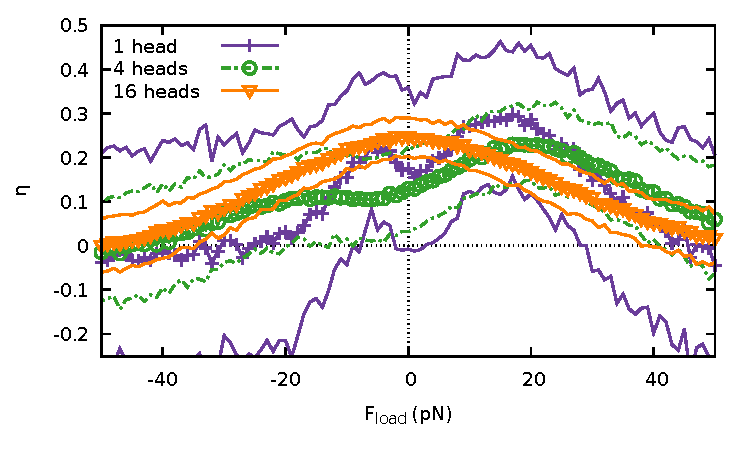
\includegraphics[width=0.45\textwidth,height=!]{chemical_cycle_1head}
\caption{
\label{fig:chem_eff_1head}
Chemical efficiency of a motor under load. 
Comparison of one (red triangles), four (blue stars), sixteen (green circles) headed motors.
We observe that with increasing number of heads the efficiency \eqref{eq:efficiency} distribution 
gets broader and it's variance decreases.
Moreover, for sixteen heads it became centered without two local maximas. 
}
\end{figure}


Another trait of the chemical efficiency curves are the local minima's around $F_\text{load}=0$. 
The understand this we must again look at equation \eqref{eq:eta} which is determined by the ratchet potential averaged with the heads' distribution in the attached and detached state. 
For a one headed motor, these distribution will both be peaked around the minimum of the ratchet potential. 
In fact, the distributions will be given by the Boltzmann distribution.
\begin{equation}
\rho(x,\zeta) = \frac{1}{Z(\zeta)} e^{-\beta \zeta V_r(x)}
\end{equation} 
From this point of view, detaching the head is equivalent to an increasing of the temperature $T\rightarrow\frac{T}{c}$. 
Hence the distributions for the detached state are broader and the expectation value of $V_r$ will be bigger than in the attached state and $\eta$ will be positive. 
Now if we apply a small external force, the distributions will be slightly perturbed and given by the McLennan formula
\begin{equation}
\rho_s^*(x) \propto e^{-\beta \left[V_r(x) - F x\right]}\propto \rho_s(x)\left[1 + \beta F x\right]
\end{equation}
which will, for small $F$, lead to a shift of the distribution $\rho_s$ along the $x$-axis and in the direction of the load. 
In the detached state this will cause a larger displacement than in the attached state because of the potential in that case is less steep. 
A larger displacement of the distribution, away from the potential's minimum, means that $\langle V_r \rangle_{s=0}$ will increase more than $\langle V_r \rangle_{s=1}$ and hence $\eta$ has to increase. 
For a four headed motor, the distributions of the heads at zero load are not exactly peaked around the minimum of the potential because of the fixed distance between each head,  which does not correspond to the period of the ratchet. 
Therefore the local minimum of $\eta$ lies not exactly at, but close to, $F_{load} =0$.
This argument can be further supported by Jensen's inequality, which follow from the fact the the ratchet potential is convex. For this case the inequality reads as follows.
\begin{equation}
V_r(\langle x \rangle) \leq \langle V_r(x) \rangle
\end{equation} 
A lower bound on the expectation value of $V_r$ is given by the value of $V_r$ at the mean position of the heads in a given state. 
In the detached state this position will be farther away from the minimum of the ratchet so the lower bound is higher than in the attached case.


\section{TO DO}
\begin{itemize}
\item Plot theoretical result for second order distribution against empirical result
\item References
\item Conclussions
\end{itemize}

\begin{acknowledgments}
Christian Maes
\end{acknowledgments}

\appendix* 
\section{Perturbative treatment}
\label{sec:perturb}
Here we show that the chemical cycle must extract energy from the ratchet system with one head and for large load forces, 
i.e. the chemical efficiency \eqref{eq:eta} must be negative. 
We will show this by calculating the perturbative corrections to the probability density of the position of the motor with respect to the actin filament, both in the ATP bound and ATP unbound state. 
For this we assume that the relaxation time of the position in a given potential is much shorter than the typical time between jumps in the chemical state of the heads. 
This will allow us to use steady state distributions to calculate the expected values of the potential energy in equation \eqref{eq:eta}.
We start with the Fokker-Planck equation for steady states, i.e. $\partial_t \rho = 0$.
\begin{equation}
\frac{1}{\gamma} \partial_x \left[ \left( F - \partial_x V_r(x) \right) \rho(x) - k_B T \partial_x \rho(x) \right] = 0
\label{eq:FP_ss}
\end{equation}
where $V$ is the ratchet potential in a given state and F is the constant load force. 
As we want to calculate perturbations for large loads we will rewrite equation \eqref{eq:FP_ss} so that we can use $\epsilon = \frac{1}{F}$ as the perturbation.
\begin{equation}
\partial_x \left[ \rho(x) - \frac{1}{F} \left( \partial_x V_r(x) \rho(x) + k_B T \partial_x \rho(x) \right) \right] = 0
\label{eq:FP_ss_pert}
\end{equation}
For infinitely large loads the steady state distribution is flat, i.e. $\rho_0 = \frac{1}{d}$, which will be the zeroth order solution. 
Since this will be the case in both the attached and detached state, it will yield the same expected values of $V$ and therefore $\eta$ must be equal to zero.
The first order solution will be of the form $\rho_1 = \rho_0 + \delta\rho_1$. 
When inserted into \eqref{eq:FP_ss_pert} and only keeping terms up to first order in $\frac{1}{F}$, we get
\begin{equation*}
\partial_x \left[ \delta \rho_1 - \frac{1}{F} \partial_x V_r(x) \rho_0 \right] = 0
\end{equation*}
or alternatively
\begin{equation*}
\delta\rho_1 = \frac{1}{dF} \partial_x V_r + C
\end{equation*}
where $C$ is an integration constant that, after normalization of $\rho_1$, must be equal to $0$.
However, this first order correction will not contribute to calculations of $\langle V_r \rangle_\rho$ since
\begin{align*}
\langle V_r \rangle_{\delta\rho_1} 
&= \int_0^d V_r(x) \, \delta\rho_1 \; \rmd x
\propto \int_0^d V_r(x) \, \partial_x V_r(x) \; \rmd x \\
&= \frac{1}{2} \int_0^d \partial_x V_r^2(x) \; \rmd x 
= 0
\end{align*}
where we used integration by parts and the fact that $V_r(x)$ is periodic.
Consequently, we need to calculate the second order correction $\delta\rho_2$. 
Now by inserting $\rho_2 = \rho_1 + \delta\rho_2$ in \eqref{eq:FP_ss_pert} and only keeping up to second order in $\frac{1}{F}$, we find
\begin{multline*}
\partial_x \left[ \delta\rho_2 - \frac{1}{F} \partial_x V_r \, \delta\rho_1 - \frac{k_B T}{F} \partial_x \delta\rho_1 \right] \\
= \partial_x \left[ \delta\rho_2 - \frac{1}{ d F^2 } \left(\partial_x V_r\right)^2 - \frac{k_B T}{dF^2} \partial_x^2 V_r \right] 
= 0
\end{multline*}
which solves to
\begin{equation*}
\delta\rho_2 = \frac{1}{ d F^2} \left[ \left( \partial_x V_r \right)^2 - k_B T \partial_x^2 V_r \right] + C^\prime.
\end{equation*}
Again by normalization, the integration constant $C^\prime$ can be determined.
\begin{multline*}
1 = \int_0^d \rho_2 \; \rmd x 
= \int_0^d \left\{ \frac{1}{d} + \frac{1}{ d F } \partial_x V_r \right\} \; \rmd x \\
+ \int_0^d \left\{  \frac{1}{ d F^2 } \left[ \left( \partial_x V_r \right)^2 - k_B T \partial_x^2 V_r \right] + C^\prime\right\} \; \rmd x 
\end{multline*}
Which simplifies to
\begin{equation}
C^\prime = - \frac{1}{ d^2 F^2 } \int_0^d \left( \partial_x V_r \right)^2 \; \rmd x . 
\end{equation}
The first order term again did not contribute and the thermal term vanished as well because of the periodicity of $V_r(x)$. 
Now the density up to second order is given by
\begin{align*}
\rho_2 =& \rho_0 + \delta\rho_1 + \delta\rho_2 \\
=& \frac{1}{d} + \frac{1}{d F} \partial_x V_r +{} \\
&+ \frac{1}{d F^2} \left[ \left( \partial_x V_r \right)^2 - k_B T \partial_x^2V_r - \frac{1}{d} \int_0^d \left( \partial_x V_r \right)^2 \; \rmd x \right] .
\end{align*}
Observe that in this form, the depends on the ratchet potential only through a first or second order derivative. 
Therefore the density will appear as a piece-wise constant function on $x\in[0,l]$, with different values for $x < a l$ and $x > a l $. 
This trend can already be seen in the empirical density obtained from simulations for large load forces $F_L = \pm 250 \, \mathrm{pN}$ in figure %TODO
%\begin{figure*}[t]
%\centering
%\subfigure[Positive load]{
%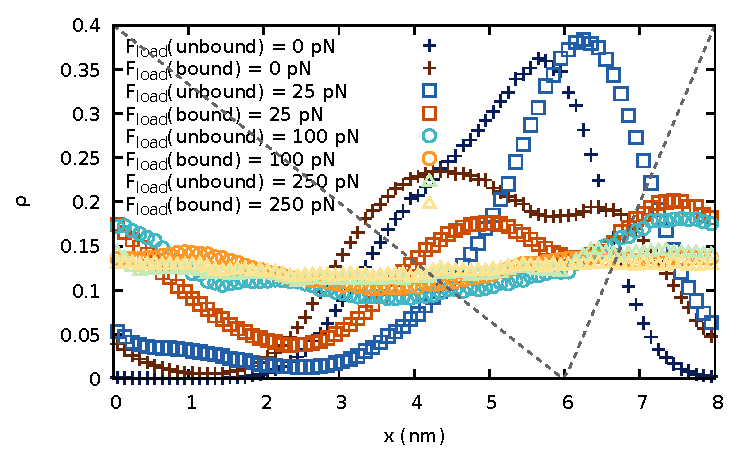
\includegraphics[width=0.45\textwidth,height=!]{pos_multiplot_p}
%}
%\subfigure[Negative load]{
%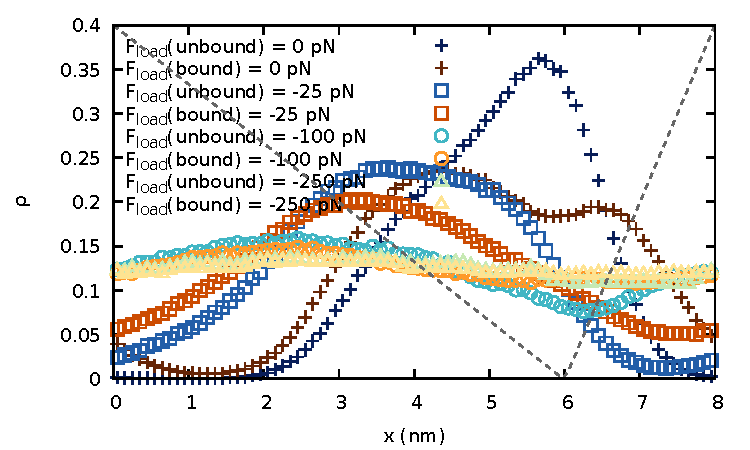
\includegraphics[width=0.45\textwidth,height=!]{pos_multiplot_m}
%}
%\caption{
%\label{fig:pos_multiplot}
%Side by side comparison of empirical density profiles in both attachable (a - blue colored) and detached (d - red colored) state for different loads.
%Profiles sharing the same load magnitude $|F_\text{load}|$ are denoted by the symbols.
%}
%\end{figure*}


With the second order correction we can now calculate the expected value of the potential energy.
\begin{align*}
\langle V_r \rangle_{\delta\rho_2} 
=& \int_0^d V_r(x) \, \delta\rho_2 \; \rmd x \\
=& \frac{1}{d F^2} \int_0^d V_r(x) \left(\partial_x V_r \right)^2 \; \rmd x  \\
&- \frac{1}{d^2 F^2} \int_0^d V_r(x) \; \rmd x \int_0^d \left( \partial_y V_r \right)^2 \; \rmd y \\
&- \frac{k_B T}{d F^2} \int_0^d V_r(x) \, \partial_x^2 V_r \; \rmd x
\end{align*}
The first two terms will cancel each other and after carrying out the integral for the third term, with $V_r(x)$ given by \eqref{eq:ratchet_potential}, one finds 
\begin{equation}
\langle V_r \rangle_{ \delta\rho_2, s=1} = \frac{k_B T}{F^2} \frac{V^2}{a \left(1-a\right) d^2 }
\end{equation}
For the expectation value in the detached state, the potentials appearing in the expression for the distributions must be re-scaled by a factor $c$, which leads to
\begin{equation}
\langle V_r \rangle_{\delta\rho_2, s=0} = \frac{k_B T}{F^2} \frac{c V^2}{a \left(1-a\right) d^2 } .
\end{equation}
Similarly, for the zeroth order expectation value we find
\begin{equation}
\langle V_r \rangle_{\rho_0} = \frac{1}{d} \int_0^d V_r(x) \; \rmd x = \frac{V}{2} .
\end{equation}
Using this, we can calculate $\eta$ up to second order in $\frac{1}{F}$. 
Note that the zeroth and first order are zero.
\begin{equation}
\eta = -\left( \frac{V}{d F} \right)^2 \frac{k_B T} { \Delta E - (1-c) \frac{V}{2} } \; \frac{ \left(1-c\right)^2 }{ a (1-a) }
\end{equation}
With this we show that, at least for a ratchet system with one motor head, it is expected that $\eta$ will become negative for large external loads and eventually goes to zero as the load goes to infinity. 
This means the driven system looses chemical energy, while the external force is performing work on the system. 
The efficiency $\eta$ is symmetric in $F$ for large forces, which is also apparent from figure \ref{fig:chem}. 
Also note that in the expression for the chemical efficiency, the ratio between the amplitude of the ratchet potential $V$ and the work done by the external force over a period of the potential $d F$ appears in the formula, as well as the ratio between the thermal energy $k_B T$ and the mean energy gap between the attached and detached state. 
Indeed for large load on the motor, the efficiency will go to zero as can be seen from the zeroth order solution.
\par
In addition we can compute the current using the obtained densities. 
The current is taken from the Fokker-Planck equation \eqref{eq:FP_ss}.
\begin{equation}
\mathcal{J} = \frac{1}{\gamma} \left[ \left( F - \partial_x V_r \right) \rho - k_B T \partial_x \rho \right] 
\end{equation}
When inserting $\rho_2$, we find the current in leading orders of $F$.
\begin{align*}
\mathcal{J} =& \frac{F}{\gamma d} \left( 1 + C^\prime \right) + \mathcal{O}( \frac{1}{F^2} ) \\
=& \frac{F}{\gamma d} - \frac{1}{F\gamma d^2} \int^d_0 \left( \partial_x V_r \right)^2 \; \rmd x + \mathcal{O}(\frac{1}{F^2}) 
\end{align*}
Important to note is that the current, integrated over the period of the ratchet, represents the mean velocity of the motor. 
Indeed, the dominant term for large external forces is $\mathcal{J}_0 = \frac{F}{\gamma}$, which was also apparent from the simulations shown in figure \ref{fig:F_v}. 
Furthermore, the force-independent term vanishes leading to an anti-symmetric form with respect to $F$. 
The first correction is given by $\frac{F}{\gamma}C^\prime\propto \frac{1}{F}$. 
This decay was clearly seen in figure \ref{fig:ratchet_force_decay}, which depicts was the mean motor velocity deduced by the drag velocity due to the load force $\frac{F}{\gamma}$. 
This isolates the contribution from the ratchet potential. 
Hence this result, obtained for a one-headed motor, also seems to hold for the simulations of motors with four heads. 

In fact, if we compare the chemical efficiencies for a motor with one head and four heads, we see a great similarity.
This comparison is made in figure \ref{fig:chem_eff_1head}.
The behavior for large load forces seems to be exactly the same.
Since $\eta$ is a ratio of chemical energies exchanged through the motor heads, this means that for large enough forces a head of the four headed motor no longer feels the presence of the other heads.
However the one headed motor is more susceptible to external forces as it's chemical efficiency starts to drop already at smaller loads. 
Note that the curves with higher detach rate $k_d$ in figure \ref{fig:chem} tend to approach the curve for one head in figure \ref{fig:chem_eff_1head}. 
When the detach rate is increased, the configuration where fewer heads of the motor are attach to the polymer indeed becomes more likely.


\bibliography{ratchet}


\end{document}
